%!TEX TS-program = xelatex
\documentclass[journal]{style/IEEEtran}
\usepackage[fontset=founder]{ctex} % 增加中文格式的支持。
%\usepackage[fontset=founder,11pt]{ctex} % 小字体,紧凑一点。

%\pdfminorversion=4

\IEEEoverridecommandlockouts                              % This command is only
                                                          % needed if you want to
                                                          % use the \thanks command
% to use ieeeconf with natbib
\makeatletter

\let\proof\@undefined
\let\endproof\@undefined

\let\NAT@parse\undefined
\makeatother 

%\usepackage{flushend}

\usepackage[numbers, sort, compress]{natbib}
\usepackage{graphicx}
\usepackage{caption}
\captionsetup{size=footnotesize,
   skip=5pt, position = bottom}
\usepackage{amsmath,amssymb}
\usepackage{amsthm} 
\usepackage{booktabs} % midrule in matrices
\usepackage[usenames,dvipsnames,svgnames,table]{xcolor}
% \usepackage[bookmarks=true,colorlinks=true,pdfpagemode=UseNone,citecolor=black,linkcolor=black,urlcolor=BrickRed,pagebackref]{hyperref}
%\usepackage{subfigure}
\usepackage{subfig} 
\usepackage{placeins}
\usepackage{algpseudocode}
% \usepackage{algorithmic}

\usepackage{multicol}
\usepackage{algorithm}

\usepackage{balance}
\usepackage{mathrsfs}

\usepackage{verbatim}
\usepackage{float}

\usepackage{style/perl_acronyms}
\usepackage{style/perl_math}
\usepackage{style/perl_SIunits}
\usepackage{style/perl_misc}

% \usepackage{color}

\usepackage[inline]{enumitem}

\newcommand{\todo}[1]{{{\bf\color{red} TODO: }\color{red}#1}}

\newcommand{\xib}[1]{\boldsymbol{\xi}_{#1}}
\newcommand{\xip}[1]{\boldsymbol{\xi}^\prime_{#1}}
\newcommand{\xic}[1]{\boldsymbol{\xi}^\curlywedge_{#1}}
\newcommand{\xipc}[1]{\boldsymbol{\xi}^{\prime\curlywedge}_{#1}}
\newcommand{\xibt}[1]{\boldsymbol{\xi}^\top_{#1}}
\newcommand{\xipt}[1]{\boldsymbol{\xi}^{\prime\top}_{#1}}
\newcommand{\xict}[1]{\boldsymbol{\xi}^{\curlywedge\top}_{#1}}
\newcommand{\xipct}[1]{\boldsymbol{\xi}^{\prime\curlywedge\top}_{#1}}

\newcommand{\mgj}[1]{[{\textbf{\textcolor{RoyalBlue}{Maani: #1}}}]}
\newcommand{\Ram}[1]{[{\textbf{\textcolor{OliveGreen}{Ram: #1}}}]}
\newcommand{\ram}[1]{[{\textbf{\textcolor{OliveGreen}{Ram: #1}}}]}


%\usepackage{hyperref}

\addtolength{\parskip}{-0.5mm}

\setlength{\textfloatsep}{0.5cm}

% correct bad hyphenation here
\hyphenation{}

% makes writing the lit review easier.  Comment this out when once it's written

% \usepackage{hyperref}

% HG: New theorem declaration. It uses less space than the original one.
\newtheoremstyle{nospace}{2pt}{1.5pt}{\itshape}{}{\bfseries}{:}{.5em}{}
\theoremstyle{nospace}
\newtheorem{theorem}{Theorem}
\newtheorem{proposition}{Proposition}
\newtheorem{corollary}{Corollary}
\newtheorem{lemma}[theorem]{Lemma}
\newtheorem{assumption}{Assumption} 
\newtheorem{remark}{Remark}
\newtheorem{definition}{Definition}

%\newcommand{\jinsun}[1]{{\normalsize{\textbf{({\color{blue}JL:\ }#1)}}}}


%\usepackage{caption}
%\captionsetup{
%  labelfont = footnotesize,
%  textfont = footnotesize,
%  skip = 1ex,  % skip the space between float and caption
%  belowskip=-10pt,
%}



\begin{document}
%\title{Characterizing the Uncertainty of Jointly Distributed Poses in the Lie~Algebra}
\title{李代数中联合分布位姿不确定性的刻画}

% author names and affiliations
% use a multiple column layout for up to three different
% affiliations
%\author{Joshua~G.~Mangelson, \textit{Student Member}, \textit{IEEE}, ~Maani~Ghaffari, \textit{Member}, \textit{IEEE},\\
%~Ram~Vasudevan, \textit{Member}, \textit{IEEE},~and~Ryan~M.~Eustice,
\author{Joshua~G.~Mangelson, ~Maani~Ghaffari, ~Ram~Vasudevan,~and~Ryan~M.~Eustice%
  \thanks{*This work was supported by the \acl{ONR} under awards
    N00014-16-1-2102. Funding for M. Ghaffari is given by the Toyota Research Institute (TRI), partly under award number N021515, however this article solely reflects the opinions and conclusions of its authors and not TRI or any other Toyota entity.}%
  \thanks{J.~Mangelson, M.~Ghaffari, R.~Vasudevan, and R.~Eustice are at the University of Michigan, Ann Arbor, MI 48109, USA. \texttt{\{mangelso, maanigj, ramv, eustice\}@umich.edu}.}  %
}

% \markboth{Journal of \LaTeX\ Class Files,~Vol.~xx, No.~xx, March~2019}%
% {Shell \MakeLowercase{\textit{et al.}}: Bare Demo of IEEEtran.cls for IEEE Journals}

% make the title area
\maketitle

\begin{abstract}
  我们分析并实验比较了用于四旋翼控制器的各种旋转误差度量。
  传统的四旋翼姿态控制器使用欧拉角或全旋转来计算姿态误差,并按比例计算控制反应。
  最近,一些研究表明,在姿态控制器中优先考虑四旋翼倾斜,或\textit{推力向量}误差,可以改善位置控制,尤其是在有大的偏航误差的情况下。
  我们提供了一个拟议的旋转度量的目录,将它们放在同一个框架中,并表明我们可以独立地推理和设计反应的量值和反应的方向。
  现有的方法主要分为两类:
    (1) 诱导最短方向的反应以校正全旋转误差的度量,以及 
    (2) 结合最短方向的反应以校正倾斜误差和在最短方向上校正偏航误差的度量。
  %We also show how linearizing the attitude dynamics can improve performance during maneuvers with large yaw error.
  %Finally, we run experiments to compare the various metrics.
  我们展示了实验结果,以突出旋转误差度量之间的显著差异。
  查看 \url{https://alspitz.github.io/roterrormetrics.html} 以交互式模拟形式可视化实验执行。
\end{abstract}

\acresetall

\IEEEpeerreviewmaketitle



\begin{figure}[t!]
    \centering
    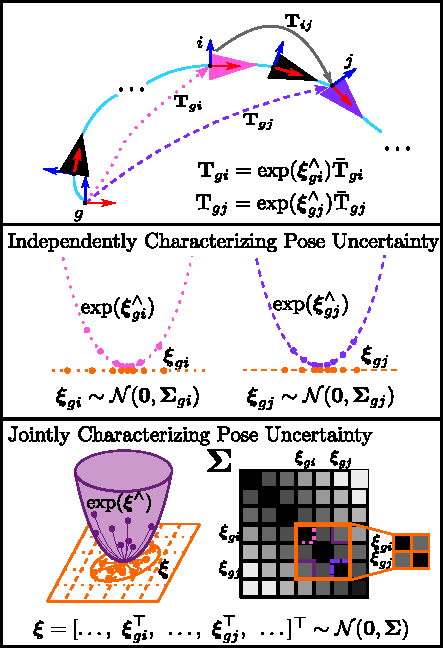
\includegraphics[width=0.9\columnwidth]{figures/main-example2.pdf}
    \caption{
    最先进的位姿图SLAM算法在每个时间步中估计机器人机体相对于固定坐标系的位姿(如上图中的 $i$ 和 $j$ ),分别用 $\mathbf{T}_{gi}$ 和 $\mathbf{T}_{gj}$ 表示。 
    在求解SLAM后,通常需要通过执行各种操作(如位姿组合、位姿求逆和相对位姿估计)来提取附加信息,同时精确地传播不确定性。
    本图顶部显示了一个相对位姿操作 $\mathbf{T}_{ij}$ 的示例。
    最近的研究已经表明,在特殊欧几里德群的李代数(如上图中所示)中,将不确定性作为高斯随机变量($\boldsymbol{\xi}_{gi}, \boldsymbol{\xi}_{gj}$)的刻画,会导致一致性的提高 \cite{barfoot2014associating};然而,这种方法的侧重于位姿组合,同时假设底层位姿是独立的。
    通常,从SLAM中估计的位姿高度相关 \cite{dissanayake2001a}。
    本文提出了一个在李代数空间中联合刻画一组相关位姿的不确定性的框架(如上图底部插图所示)。 
    然后描述了如何在此框架内执行位姿组合、位姿求逆和相对位姿操作。}
    \label{fig:main_example}
\end{figure}

\section{序言}

机器人位姿(位置和方向)不确定性的精确刻画对于鲁棒的长期的自主性至关重要,因为规划和安全决策通常基于它们的数值 \cite{thrun2005probabilistic}。例如,过于自信的位置估计可能导致自动驾驶汽车驶出车道或水下航行器与水下建筑相撞。另一方面,信心不足会导致行动迟缓。  

最早刻画坐标帧关系的位姿不确定性的论文之一,使用多元高斯参数向量和相关协方差矩阵来表示物体的相对位姿 \cite{smith1986a}。 
这篇论文后来被Smith、Self和Cheesman \cite{smith1990a} 扩展,将多个不确定的空间关系表示为一个可用于评估任意给定位姿相对于任意其它位姿的不确定性的随机映射(\textit{stochastic map})。 
他们还提出了几种操作(如 \figref{fig:main_example} 所示的相对位姿操作),这些操作能够提取不直接估计的附加信息,以及通过这些操作基于一阶坐标的方法传播不确定性。 
% These methods had a significant effect on the field and have been widely used since. 
为简洁起见,在文献 \cite{smith1990a} 中提出的操作通常由论文作者的首字母 (SSC) 表示。 



尽管众所周知,刚体变换(或 $\mathbb{R}^3$ 的运动群)是由三维(3D)特殊欧几里德群~\citep{spong2005robot,murray1994mathematical},$\mathrm{SE}(3)$ 描述的,这些变换的不确定性通常在局部坐标系中建模,从而导致在估计问题~\citep{huang2007convergence}中的不一致性或在不确定性传播~\citep{rodriguez2018importance}中的单调性损失。\citet{wang2008nonparametric} 和 \citet{long2013banana} 通过使用位于 $\mathrm{SE}(d)$ 的李代数中的指数坐标(\emph{exponential coordinates})来表示每个位姿,能够克服这些问题。 
 
\citet{barfoot2014associating} 证明了通过直接在李代数中对不确定性进行建模,然后使用指数映射在群空间中诱导分布,可以简化传播计算。 
由于李代数是一个向量空间,一个小的扰动项可以在 $\mathbb{R}^6$ 中建模为零均值高斯噪声,然后用于扰动群空间中的平均(或标称)位姿。 
文献 \cite{barfoot2014associating} 然后在此基础上,推导出当相关位姿独立时位姿组合操作的一阶和二阶不确定性传播。 
我们对一组位姿的不确定性进行建模的方法与此类似,但是我们放弃了独立性要求,因为由SLAM估计的位姿很少独立,并且它还附加描述了位姿求逆和相对位姿提取的附加操作(参见 \figref{fig:main_example})。 

本文的主要贡献如下:
\begin{enumerate}
    \item 我们提出了一个框架,描述了如何表示联合相关的位姿,同时使用李代数来刻画不确定性;
    \item 我们推导了所提议的框架与SSC操作的等价性;
    \item 我们描述了如何从替代的不确定性刻画参数化转换到所提议的框架(包括从MLE的解中提取李代数协方差);而且, 
    \item 我们发布了一个配套的C++库实现,以及这里介绍的例子。
\end{enumerate}
本文的其余部分组织如下:
第 \ref{sec:SE3} 节简要介绍了特殊欧几里德群及其在李群理论中的一些必要概念。 
第 \ref{sec:SSC} 节提供了SSC不确定性表示框架及其相关操作的摘要。 
第 \ref{sec:lie_joint_uncertainty} 节描述如何使用李代数来描述联合分布位姿的不确定性。 
第 \ref{sec:pose_composition}, \secref{sec:inverse}, 和 \secref{sec:relative_pose} 节分别描述了位姿组合、位姿求逆和相对位姿操作的推导,以及在李代数上不确定性的刻画。
第 \ref{sec:conversion} 节描述了如何从基于坐标系的不确定性表示转换为基于李代数的不确定性表示,以及如何从MLE的解中提取位姿不确定性的估计。
第 \ref{sec:eval} 节描述了所提议的方法的实验评估。
第 \ref{sec:library} 节描述了已发布的代码库的实现。 
最后, 第 \ref{sec:conclusion} 节总结全文。 

%\input{problem_formulation}
\section{特殊欧几里德群与李群理论}
\label{sec:SE3}

空间中物体或坐标系之间的相对位姿(位置和方向)估计是机器人导航、感知和操纵中的一个常见问题。 
形式上,我们将三维相对位姿变换表示为特殊欧几里德群(\textit{Special Euclidean group})的元素。 
本节简要介绍特殊欧几里德群(\textit{Special Euclidean group})和李群理论的相关内容,这些内容在随后的推导和讨论中非常重要。  

\subsection{特殊欧几里德群}



特殊欧几里德群(\textit{Special Euclidean group}),或 $\mathrm{SE}(d)$,表示齐次变换矩阵的空间,或者将刚体旋转和平移应用于 $\mathbb{R}^d$(以齐次形式表示)中的点的矩阵空间。 
形式上,在三维中,$\mathrm{SE}(3)$ 定义如下:
\begin{equation}
    \mathrm{SE}(3) := \left\{ \mathbf{T} = \left[ \begin{array}{cc}
        \mathbf{R}~ & \mathbf{t} \\
        \mathbf{0}^\top & 1
    \end{array} \right] \in \mathbb{R}^{4 \times 4} \middle| \mathbf{R} \in \mathrm{SO}(3), \mathbf{t} \in \mathbb{R}^3\right\},
\end{equation}
其中 $\mathrm{SO}(3)$ 是特殊正交群(\textit{Special Orthogonal group}),它是有效旋转矩阵的空间: 
\begin{equation}
    \mathrm{SO}(3) := \left\{ \mathbf{R} \in \mathbb{R}^{3 \times 3} | \mathbf{R}\mathbf{R}^\top = \mathbf{I}_3, \operatorname{det}\mathbf{R} = 1 \right\},~~~
\end{equation}
并且 $\mathbf{I}_d$ 是维度为 $d$ 的单位矩阵。 
现在已经发展了多种方法来参数化这些对象,例如欧拉角或四元数 \cite{spong2005robot}。  

$\mathrm{SE}(3)$ 和 $\mathrm{SO}(3)$ 都是矩阵李群(\textit{Lie groups}),这意味着它们是平滑流形,也满足数学群~\cite{tapp2016matrix,baker2012matrix}的形式定义与标准矩阵乘法操作。 
直观地说,这意味着虽然一般的群是非线性的,但每一个群都可以用欧几里德向量空间进行局部近似。 
此外,对于流形上的任意给定点,考虑流形上通过该点的所有路径的集合。 
在给定点上的所有路径的速度(方向和速度的项)的集合构成一个称为切空间的向量空间。 
以幺元为中心的切空间称为Lie代数(\textit{Lie algebra})。 
这种关系在 \figref{fig:lie_algebra} 中被描绘出来。 

$\mathrm{SO}(3)$ 的李代数表示为 $\mathfrak{so}(3)$ ,并且是斜对称的$3\times3$矩阵空间~\cite{chirikjian2011stochastic,tapp2016matrix}: 
\begin{equation}
    \mathfrak{so}(3) := \left\{ \boldsymbol{\omega} \in \mathbb{R}^{3 \times 3} ~| ~\boldsymbol{\omega}^\top = - \boldsymbol{\omega}\}\right.~~~
\end{equation}
这个空间同构于 $\mathbb{R}^3$ ,因为斜对称矩阵的对角项上为零,而下项完全由三个上项标识(因此 $\mathrm{dim}~\mathfrak{so}(3) = 3$)。因此,改为使用 $\mathbb{R}^3$ 非常方便。 
注意,我们可以使用 $\wedge$ 算子获取 $\mathbb{R}^3$ 的元素并将其转换为 $\mathfrak{so}(3)$ 的元素: 
\begin{equation}
    \boldsymbol{\phi}^\wedge := \left[ \begin{array}{c}
         \phi_{1} \\
         \phi_{2} \\
         \phi_{3}
    \end{array} \right]^\wedge = 
    \left[ \begin{array}{ccc}
        0 & -\phi_{3} & \phi_{2} \\
        \phi_{3} & 0 & -\phi_{1} \\
        -\phi_{2} & \phi_{1} & 0
    \end{array} \right] \in \mathfrak{so}(3),
\end{equation}
%\begin{equation}
%    \boldsymbol{\phi}_\ell^\wedge := \left[ \begin{array}{c}
%         \phi_{\ell,1} \\
%         \phi_{\ell,2} \\
%         \phi_{\ell,3}
%    \end{array} \right]^\wedge = 
%    \left[ \begin{array}{ccc}
%        0 & -\phi_{\ell,3} & \phi_{\ell,2} \\
%        \phi_{\ell,3} & 0 & -\phi_{\ell,1} \\
%        -\phi_{\ell,2} & \phi_{\ell,1} & 0
%    \end{array} \right].
%\end{equation}
其中 $\boldsymbol{\phi} \in \mathbb{R}^3$。
$\vee$ 算子表示 $\wedge$ 的逆运算。 

类似地,$\mathrm{SE}(3)$ 或 $\mathfrak{se}(3)$ 的李代数定义如下: 
\begin{equation}
    \mathfrak{se}(3) := 
    \left\{ \left[ \begin{array}{cc}
        \boldsymbol{\omega} & \boldsymbol{\rho}  \\
        \mathbf{0}^\top & 0
    \end{array} \right]~ \middle| ~\boldsymbol{\omega} \in \mathfrak{so}(3), \boldsymbol{\rho} \in \mathbb{R}^3 \right\}.
\end{equation}
这个矩阵空间同构于 $\mathbb{R}^6$ ,我们重载 $\wedge$ 算子以在欧几里德向量和矩阵形式之间进行转换: 
\begin{equation}
    \boldsymbol{\xi}^\wedge := \left[ \begin{array}{c}
         \boldsymbol{\rho} \\
          \boldsymbol{\phi}
    \end{array} \right]^\wedge = 
    \left[ \begin{array}{cc}
        \boldsymbol{\phi}^\wedge & \boldsymbol{\rho}  \\
        \mathbf{0}^\top & 0
    \end{array} \right] \in \mathfrak{se}(3),
\end{equation}
%\begin{equation}
%    \boldsymbol{\xi}^\wedge := \left[ \begin{array}{c}
%         \boldsymbol{\rho}_\ell \\
%          \boldsymbol{\phi}_\ell
%    \end{array} \right]^\wedge = 
%    \left[ \begin{array}{cc}
%        \boldsymbol{\phi}_\ell^\wedge & \boldsymbol{\rho}_\ell  \\
%        \mathbf{0}^\top & 0
%    \end{array} \right]
%\end{equation}
其中 $\boldsymbol{\xi} \in \mathbb{R}^6$ 并且 $\boldsymbol{\rho}, \boldsymbol{\phi} \in \mathbb{R}^3$。

理解该群空间和代数空间之间的关系可以使我们利用该代数是向量空间这一事实。 
接下来的几个小节将介绍李群理论中的一些重要概念,这些概念我们将在本文的其余部分用到。 
在此过程中,我们使用 $\mathcal{G}$ 表示给定的李群,并使用 $\mathfrak{g}$ 表示其关联的李代数。 

\begin{figure}[t]
    \centering
    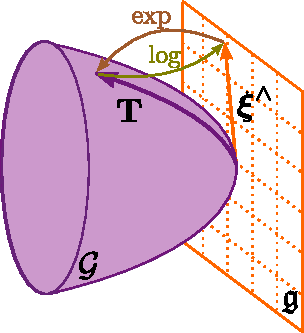
\includegraphics[width=0.7\columnwidth]{figures/lie-group-example.pdf}
    \caption{
    % An illustration of the relationship between a Lie group $\mathcal{G}$ and its associated Lie algebra $\mathfrak{g}$.
    李代数,$\mathfrak{g}$,是以幺元元素为中心的李群 $\mathcal{G}$ 的切空间。 
    李代数表示一个粒子在群上某一给定点所能达到的所有可能速度的空间。 
    指数映射(\textit{exponential map})将李代数中的速度,$\boldsymbol{\xi}^\wedge \in \mathfrak{g}$,映射到它们在李群中的相关作用,$\mathbf{T} \in \mathcal{G}$,而对数映射(\textit{logarithm map})执行逆操作。}
    \label{fig:lie_algebra}
\end{figure}

\subsection{指数映射}

李代数,$\mathfrak{g}$,表示流形在幺元处的切空间。 
但是,给定一个特定的切向量,我们可能需要将其转换为群空间$\mathcal{G}$中与其相关联的变换。 
指数映射(\textit{exponential map}), $\operatorname{exp} : \mathfrak{g} \rightarrow \mathcal{G}$,(对于 $\mathrm{SE}(3)$ 可以以封闭形式定义),使我们能够执行此转换,
\begin{equation}
    \operatorname{exp}(\boldsymbol{\xi}^\wedge) = \sum^\infty_{k=0} \frac{ (\boldsymbol{\xi}^\wedge)^k }{k!} = \mathbf{I}_4 + \boldsymbol{\xi}^\wedge + \frac{(\boldsymbol{\xi}^\wedge)^2}{2} + \cdots.
\end{equation}
对数映射(\textit{logarithm map}),$\operatorname{log} : \mathcal{G} \rightarrow \mathfrak{g}$,另一方面,使我们能够从另一个方向,从群空间中的作用/变换到诱导它的速度, 
\begin{equation}
    \operatorname{log}(\mathbf{T}) = \sum^\infty_{k=1} (-1)^{k+1} \frac{(\mathbf{T} - \mathbf{I}_4)^k}{k}.
\end{equation}
这种关系在 \figref{fig:lie_algebra} 中得到了可视化。 

\subsection{伴随作用}

假设 $\mathbf{T} \in \mathcal{G}$ 和 $\boldsymbol{\xi} \in \mathfrak{g}$, 则 $\mathbf{T}$ 对于 $\boldsymbol{\xi}$ 的伴随作用, 或 $\operatorname{Ad}_\mathbf{T}(\boldsymbol{\xi})$ 的定义如下:
\begin{equation}
    \operatorname{Ad}_\mathbf{T}(\boldsymbol{\xi}) := \operatorname{Ad}_\mathbf{T} \boldsymbol{\xi} = \operatorname{log}( \mathbf{T} \operatorname{exp} ( \boldsymbol{\xi} ) \mathbf{T}^{-1} ).
\end{equation}
伴随作用描述了对于李代数的一个元素,应用左变换和它的右逆,将其变换到群空间的影响。 
这就产生了以下属性,我们在后面会使用到: 
\begin{align}
    % \mathbf{T} \operatorname{exp} ( \boldsymbol{\xi} ) \mathbf{T}^{-1} = \operatorname{exp} ( \operatorname{Ad}_\mathbf{T} \boldsymbol{\xi} ) \\
    \mathbf{T} \operatorname{exp} ( \boldsymbol{\xi} ) = \operatorname{exp} ( \operatorname{Ad}_\mathbf{T} \boldsymbol{\xi} ) \mathbf{T} \label{eq:adjoint_property}
\end{align}

%There are also times where we want to understand the effect that applying a coordinate transformation in the group space has on an element of the algebra \Ram{this is a fairly vague description of the effect the adjoint captures.}. 
%The \textit{adjoint action} characterizes this effect. 
%Assuming $\mathbf{T} \in \mathcal{G}$ and $\boldsymbol{\xi} \in \mathfrak{g}$, the adjoint action of $\mathbf{T}$ on $\boldsymbol{\xi}$, or $\operatorname{Ad}_\mathbf{T}(\boldsymbol{\xi})$ is defined as follows:
%\begin{equation}
%    \operatorname{Ad}_\mathbf{T}(\boldsymbol{\xi}) := \operatorname{Ad}_\mathbf{T} \boldsymbol{\xi} = \operatorname{log}( \mathbf{T} \operatorname{exp} ( \boldsymbol{\xi} ) \mathbf{T}^{-1} ),
%\end{equation}
%where $\operatorname{Ad}_\mathbf{T}$ is the matrix representation of the action \cite{chirikjian2011stochastic}.
%This gives rise to the following property, which we use later on:
%\begin{align}
    % \mathbf{T} \operatorname{exp} ( \boldsymbol{\xi} ) \mathbf{T}^{-1} = \operatorname{exp} ( \operatorname{Ad}_\mathbf{T} \boldsymbol{\xi} ) \\
%    \mathbf{T} \operatorname{exp} ( \boldsymbol{\xi} ) = \operatorname{exp} ( \operatorname{Ad}_\mathbf{T} \boldsymbol{\xi} ) \mathbf{T} \label{eq:adjoint_property}
%\end{align}
% \Ram{this last equation is awkwardly typeset. I would just explain that by taking the exp on both sides of (9) and then multiplying by T on the RHS of both sides you get (11).}

\subsection{Baker-Campbell-Hausdorff (BCH) 公式}

最后,我们还想刻画群空间中的乘法对李代数的影响。 
更具体地,假设我们要计算李代数元素,$\boldsymbol{\xi}_{ac}\in \mathfrak{g}$,它是通过取两个李代数 $\boldsymbol{\xi}_{ab}, \boldsymbol{\xi}_{bc} \in \mathfrak{g}$ 的指数的乘积的对数产生的。 
% given two elements of the Lie algebra $\boldsymbol{\xi}_{ab}, \boldsymbol{\xi}_{bc} \in \mathfrak{g}$, we want to understand what the resulting Lie algebra element $\boldsymbol{\xi}_{ac}\in \mathfrak{g}$ looks like if we multiply the associated group actions of $\boldsymbol{\xi}_{ab}$ and $\boldsymbol{\xi}_{bc}$ then convert back to the Lie algebra space.
 \textit{Baker-Campbell-Hausdorff (BCH)} 公式纯粹是在李代数空间中描述这种关系,而不需要应用指数或对数:
\begin{align}
    \boldsymbol{\xi}_{ac} &= 
    \operatorname{log}( \operatorname{exp}(\boldsymbol{\xi}_{ab}) \operatorname{exp}(\boldsymbol{\xi}_{bc})) \label{eq:BCH}\\
    &= \boldsymbol{\xi}_{ab} + \boldsymbol{\xi}_{bc} + \frac{1}{2}[\boldsymbol{\xi}_{ab}, \boldsymbol{\xi}_{bc}] + \nonumber \\ 
    & + \frac{1}{12}([\boldsymbol{\xi}_{ab}, [\boldsymbol{\xi}_{ab}, \boldsymbol{\xi}_{bc}]] + [\boldsymbol{\xi}_{bc},[\boldsymbol{\xi}_{bc},\boldsymbol{\xi}_{ab}]]) + \cdots\nonumber,
\end{align}
其中 $[\cdot, \cdot]$ 是 $\mathfrak{g}$ \cite[(7.18)]{barfoot2017state} 的李括号。 
为简洁起见,在我们考虑 $\mathrm{SE}(3)$ 中的元素的特殊情况下,我们采用了文献 \cite{barfoot2014associating} 的符号: 
\begin{equation}
    \boldsymbol{\xi}_i^\curlywedge := \left[ \begin{array}{c}
         \boldsymbol{\rho}_i \\
          \boldsymbol{\phi}_i
    \end{array} \right]^\curlywedge = 
    \left[ \begin{array}{cc}
        \boldsymbol{\phi}_i^\wedge & \boldsymbol{\rho}_i^\wedge  \\
        \mathbf{0} &  \boldsymbol{\phi}_i^\wedge
    \end{array} \right],
\end{equation}
这允许我们将BCH公式写成:
\begin{align}
    \xib{ac} &= \xib{ab} + \xib{bc} + \frac{1}{2}\xic{ab}\xib{bc} + \frac{1}{12}\xic{ab}\xic{ab}\xib{bc} + \frac{1}{12}\xic{bc}\xic{bc}\xib{ab} \nonumber\\
    &- \frac{1}{24}\xic{bc}\xic{ab}\xic{ab}\xib{bc} + \dots. \label{eq:BCH_SE3}
\end{align}

\subsection{定义位姿上的随机变量}

最后,正如文献 \cite{barfoot2014associating} 中所讨论的,我们可以为 $\mathrm{SE}(3)$ 定义随机变量,根据 
\begin{equation}
    \mathbf{T}_\ell := \operatorname{exp}(\boldsymbol{\xi}_\ell^{\wedge}) \bar{\mathbf{T}}_\ell
    \label{eq:T_i}
\end{equation}
其中 $\bar{\mathbf{T}}_\ell\in \mathrm{SE}(3)$ 是一个 `大的' 无噪声值,而 $\boldsymbol{\xi}_\ell \in \mathbb{R}^6$ 是一个 `小的' 噪声扰动 (使用文献 \cite{barfoot2014associating} 的命名法)。
这种噪声扰动的两个例子在 \figref{fig:main_example} 的中间一行描述。 
通过定义 $\boldsymbol{\xi}_\ell$ 为在李代数中的零均值高斯随机变量 $\boldsymbol{\xi}_\ell \sim \mathcal{N}(\mathbf{0}, \boldsymbol{\Sigma}_\ell)$,我们在 $\mathrm{SE}(3)$ 上诱导出一个概率分布函数,该概率分布函数用定义于李代数 \cite{barfoot2014associating} 的均值 $\bar{\mathbf{T}}_\ell \in \mathrm{SE}(3)$ 和协方差 $\boldsymbol{\Sigma}_\ell$ 参数化。 

我们在第 \ref{sec:lie_joint_uncertainty},\ref{sec:pose_composition},\ref{sec:inverse},和 \ref{sec:relative_pose} 节中提议了一个联合相关位姿建模框架,并为 \figref{fig:summary} 中的操作推导了不确定性传播方程。不管怎样,我们首先回顾基于SSC坐标的方法。 

\begin{figure*}[t]
    \centering
    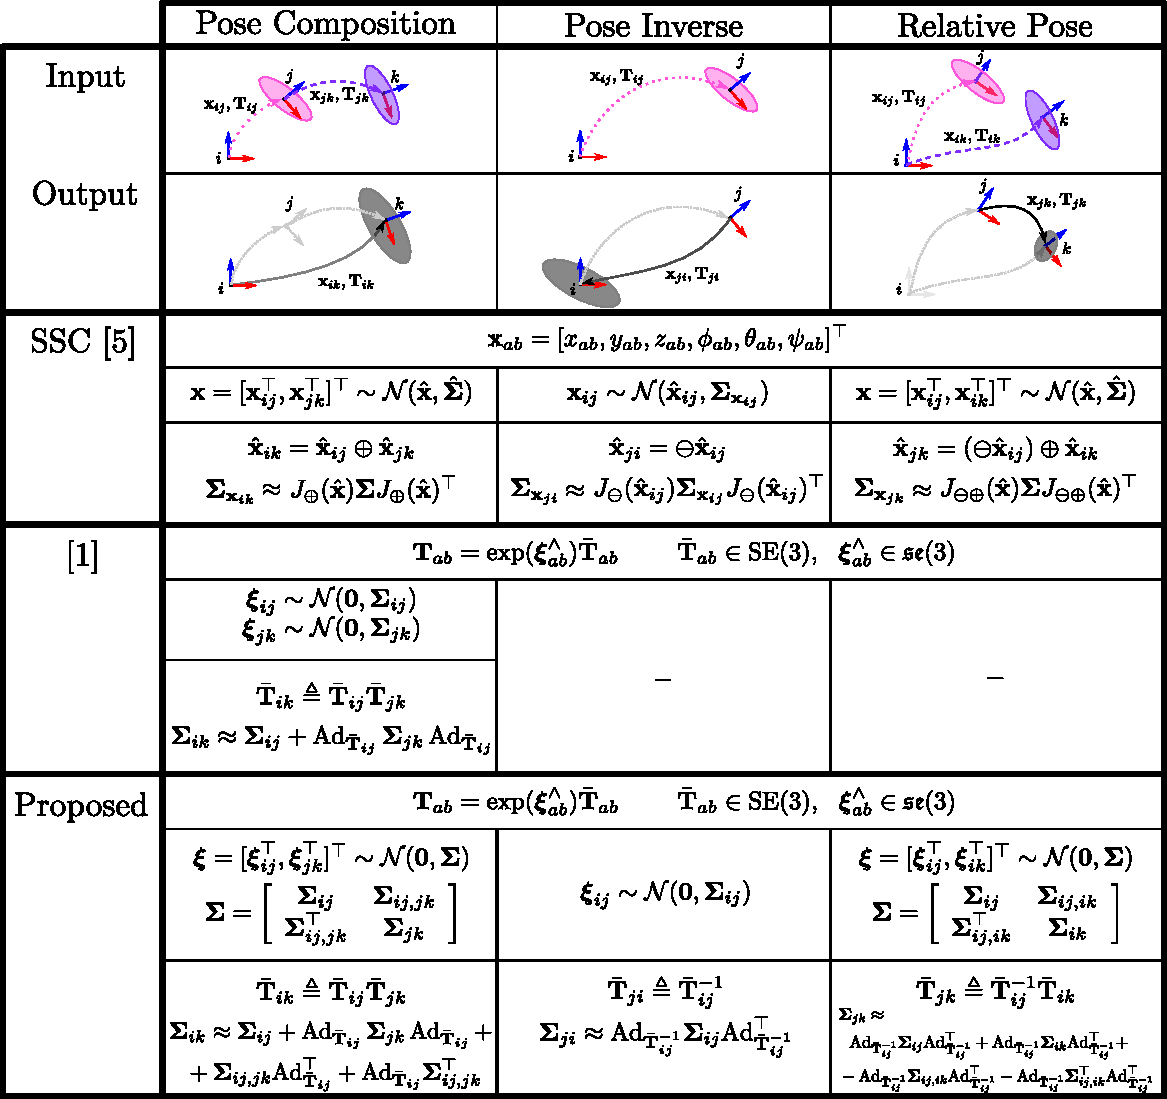
\includegraphics[width=\textwidth]{figures/Lie-SSC-Operations-Summary.pdf}
    \caption{
    总结 \citet{smith1990a}, \citet{barfoot2014associating} 和本文提出的位姿组合、位姿求逆和相对位姿操作及其相应的不确定性传播方法。索引 $i$, $j$ 和 $k$ 对应于机器人机体在不同的时间步长或位置的特定坐标系。 
    SSC \cite{smith1990a} 使用欧拉角向量和平移参数 $\mathbf{x}_{ab}$ 参数化帧 $b$ 相对于帧 $a$ 的位姿。然后,他们用均值 $\hat{\mathbf{x}}$ 和协方差 $\boldsymbol{\Sigma}$ 的多元高斯分布来建模这个参数向量。在此模型下,他们推导了位姿组合、位姿求逆和相对位姿操作的一阶不确定性传播方程。然而,由于参数向量 $\mathbf{x}_{ab}$ 不是真正的高斯分布,这种基于坐标的参数化无法精确地建模位姿不确定性。 
    \citet{barfoot2014associating} 替换帧 $b$ 相对于帧 $a$ 的位姿参数化,使用特殊欧几里德群的均值元素,$\bar{\mathbf{T}}_{ab}$,以及定义在李代数 $\mathfrak{se}(3)$中的不确定扰动或噪声参数 $\boldsymbol{\xi}_{ab}^\wedge$。这使得他们能够使用高斯分布来建模 $\boldsymbol{\xi}_{ab}$,并精确地考虑到该群的非线性结构。然而,文献 \cite{barfoot2014associating} 假设位姿是独立的,并且主要关注位姿组合操作。 
    本文的主要贡献(\textbf{primary contribution})是将 \citet{barfoot2014associating} 所提议的方法推广到联合相关位姿,并推导出位姿求逆和相对位姿操作,同时利用李代数来刻画不确定性。} 
    \label{fig:summary}
\end{figure*}

\FloatBarrier

\section{对SSC的回顾}
\label{sec:SSC}

随机映射由 \citet{smith1990a} 提出,它由多个不确定的空间关系组成,这些空间关系被视为联合高斯多元随机变量,并使用位置和欧拉角的均值向量以及相关的协方差矩阵进行参数化。\citet{smith1990a} 还提出三种操作,可以从这个映射中提取可能无法直接估计的信息。 
这三种操作是位姿组合(在文献\cite{smith1990a}中为头到尾(head-to-tail))、位姿求逆和相对位姿估计(在文献\cite{smith1990a}中为尾到尾(tail-to-tail)),如 \figref{fig:summary} 所示。本节回顾在文献 \cite{smith1990a} 中制定的位姿表示和SSC操作。 

%\FloatBarrier

\subsection{位姿表示与随机映射(\textit{Stochastic Map})}

在SSC符号下,坐标系 $i$ 和 $j$ 之间的相对变换,或坐标系 $j$ 相对于坐标系 $i$ 的位姿,被表示为 
\begin{equation}
    \mathbf{x}_{ij} = [x_{ij}, y_{ij}, z_{ij}, \phi_{ij}, \theta_{ij}, \psi_{ij}]^\top, \label{eq:SSC_rep}
\end{equation}
其中 $x_{ij}$、 $y_{ij}$、和 $z_{ij}$ 是位置坐标,并且 $\phi_{ij}$、 $\theta_{ij}$、和 $\psi_{ij}$ 是Euler角度,这些是坐标系 $j$ 相对于坐标系 $i$ 的位置和方向的编码。 
然而,由于每个相对变换都是从噪声测量中导出的,因此我们的估计是不确定的,并且我们不知道 $\mathbf{x}_{ij}$ 的真实值。 
相反,我们跟踪其参数的标称均值和相关的 $6\times 6$ 协方差矩阵,分别是 $\hat{\mathbf{x}}_{ij}$ 和 $\boldsymbol{\Sigma}_{\mathbf{x}_{ij}}$。 

随机映射(\textit{Stochastic Map}),在文献\cite{smith1990a}中提出,将所有的不确定变换视为联合高斯多元随机变量,将它们堆叠成单一的状态向量 $\mathbf{x}$,并跟踪该状态的均值和协方差。 
假设我们有 $n$ 个相对变换需要跟踪,如果我们从 $a=1, \dots, n$ 索引它们,那么 $\mathbf{x}$ 及其相关的均值和协方差是: 
\begin{align}
\mathbf{x} &= 
    \left[ \begin{array}{c} 
        \mathbf{x}_1 \\ \vdots \\ \mathbf{x}_n \end{array} \right],
\hat{\mathbf{x}} =       
    \left[ \begin{array}{c} 
        \hat{\mathbf{x}}_1 \\ \vdots \\ \hat{\mathbf{x}}_n \end{array} \right], 
\hat{\boldsymbol{\Sigma}} =       
    \left[ \begin{array}{ccc} 
        \boldsymbol{\Sigma}_{\mathbf{x}_1} & \dots & \boldsymbol{\Sigma}_{\mathbf{x}_1 \mathbf{x}_n} \\
        \vdots & \ddots & \vdots \\
        \boldsymbol{\Sigma}_{\mathbf{x}_n \mathbf{x}_1} & \dots  & \boldsymbol{\Sigma}_{\mathbf{x}_n} \\
        \end{array}\right] \label{eq:SSC_joint_rep}
\end{align}
其中, $\mathbf{x}$ 是长度为 $6n$ 的向量,$\boldsymbol{\Sigma}_{\mathbf{x}_a}$ 是相对变换 $\mathbf{x}_a$ 的 $6\times6$ 协方差矩阵,并且形式为 $\boldsymbol{\Sigma}_{\mathbf{x}_a \mathbf{x}_b}$ 的非对角块分别是 $6\times6$ 交叉协方差矩阵。 

\subsection{位姿组合(头到尾)}
\label{sec:SSC:head-to-tail}

假设我们对机器人在时间步长 $i$ 和 $j$ $(\mathbf{x}_{ij})$ 之间的相对位姿进行了噪声观测,并对其在时间步长 $j$ 和 $k$ $(\mathbf{x}_{jk})$ 之间的相对位姿进行了另一个噪声观测,我们可能想通过组合观测值 $\mathbf{x}_{ij}$ 和 $\mathbf{x}_{jk}$ 来计算时间步长 $i$ 和 $k$ $(\mathbf{x}_{ik})$ 之间的相对位姿(参见 \figref{fig:summary})。 
SSC的头到尾(\textit{head-to-tail})操作是一个非线性函数 $f_\oplus: \mathbb{R}^{6} \times \mathbb{R}^6 \rightarrow \mathbb{R}^6$,它将参数向量 $\mathbf{x}_{ij}$ 和 $\mathbf{x}_{jk}$ 做为输入,并输出参数向量 $\mathbf{x}_{ik}$,这是由各自的齐次变换矩阵组合的结果。 
$\oplus$ 算子表示这种操作: 
\begin{equation}
    \mathbf{x}_{ik} \triangleq \mathbf{x}_{ij} \oplus \mathbf{x}_{jk} = f_\oplus(\mathbf{x}_{ij}, \mathbf{x}_{jk}).
\end{equation}
由此产生的位姿的均值和协方差估计是一阶方程,为 
\begin{equation}
    \hat{\mathbf{x}}_{ik} = \hat{\mathbf{x}}_{ij} \oplus \hat{\mathbf{x}}_{jk}
\end{equation}
并且 
\begin{equation}
    \boldsymbol{\Sigma}_{\mathbf{x}_{ik}} \approx J_\oplus(\hat{\mathbf{x}}_{ij}, \hat{\mathbf{x}}_{jk}) ~ \hat{\boldsymbol{\Sigma}} ~
    J_\oplus(\hat{\mathbf{x}}_{ij}, \hat{\mathbf{x}}_{jk})^\top
\end{equation}
其中 $J_\oplus(\hat{\mathbf{x}}_{ij}, \hat{\mathbf{x}}_{jk})$ 是 $f_\oplus$ 在 $\hat{\mathbf{x}}_{ij}$ 和 $\hat{\mathbf{x}}_{jk}$ 处的 Jacobian 矩阵,并且 
\begin{align}
    \hat{\boldsymbol{\Sigma}} 
    &= 
    \left[ \begin{array}{cc}
        \boldsymbol{\Sigma}_{
        \mathbf{x}_{ij}} & ~~~\boldsymbol{\Sigma}_{\mathbf{x}_{ij}\mathbf{x}_{jk}}  \\
        ~~~\boldsymbol{\Sigma}_{\mathbf{x}_{ij}\mathbf{x}_{jk}}^\top & \boldsymbol{\Sigma}_{\mathbf{x}_{jk}}
    \end{array} \right]. 
\end{align} 

\subsection{位姿求逆}
\label{sec:SSC:inverse}

假设我们有一个机器人机体,它的任务是在一个先验的(\textit{a priori})未知的环境中导航,之后必须返回原点。 
虽然使用估计理论来表示机器人机体相对于原点的当前位置是常见的,但是代替原点表示,用相对于局部机器人坐标系来刻画位姿可能更有用。 
形式上,给定坐标帧 $j$ 相对于帧 $i$ ($\mathbf{x}_{ij}$) 的位姿的不确定估计,我们要确定帧 $i$ 相对于帧 $j$ ($\mathbf{x}_{ji}$) 的位姿。 
这相当于找到向量 $\hat{\mathbf{x}}_{ji}$,它对应于 $\hat{\mathbf{x}}_{ij}$ 的求逆(用齐次变换矩阵表示),并表示关于这个新参照系的不确定性。 

SSC 的位姿求逆(\textit{pose inverse})操作是一个非线性函数 $f_\ominus: \mathbb{R}^6 \rightarrow \mathbb{R}^6 $,它获取位姿并将该位姿求逆计算为齐次变换矩阵: 
\begin{equation}
    \mathbf{x}_{ji} \triangleq \ominus \mathbf{x}_{ij} = f_\ominus(\mathbf{x}_{ij}).
\end{equation}
由此产生的位姿的均值和协方差估计是一阶方程,为
\begin{equation}
    \hat{\mathbf{x}}_{ji} = \ominus \hat{\mathbf{x}}_{ij} 
\end{equation}
并且 
\begin{equation}
    \boldsymbol{\Sigma}_{\mathbf{x}_{ji}} \approx J_\ominus(\hat{\mathbf{x}}_{ij}) ~ \boldsymbol{\Sigma}_{\mathbf{x}_{ij}} ~
    J_\ominus(\hat{\mathbf{x}}_{ij})^\top
\end{equation}
其中 $J_\ominus(\hat{\mathbf{x}}_{ij})$ 是 $f_\ominus$ 在 $\hat{\mathbf{x}}_{ij}$ 处的 Jacobian 矩阵。

\subsection{相对位姿(尾到尾)}
\label{sec:SSC:tail-to-tail}

最后,SSC的尾到尾(\textit{tail-to-tail})操作对两个坐标帧相对于单个原点帧进行不确定估计,并评估它们之间的相对位姿。 
更简洁地说,给定 $\mathbf{x}_{ij}$ 和 $\mathbf{x}_{ik}$,找到 $\mathbf{x}_{jk}$。 
当使用位姿图同步定位和建图(pose graph \ac{SLAM})方法进行导航时,此操作非常有用,因为机器人在多个时间步长的位姿通常是相对于单个固定坐标系估计的。

SSC的相对位姿(\textit{relative pose})操作是一个非线性函数 $f_{\ominus\oplus}: \mathbb{R}^6 \times \mathbb{R}^6 \rightarrow \mathbb{R}^6$,它由首先应用位姿求逆操作,然后应用位姿组合(head-to-tail)操作来定义: 
\begin{equation}
    \mathbf{x}_{jk} \triangleq (\ominus \mathbf{x}_{ij}) \oplus \mathbf{x}_{ik} = f_{\ominus\oplus}(\mathbf{x}_{ij}, \mathbf{x}_{ik}).
\end{equation}
由此产生的位姿的均值和协方差估计是一阶方程,为
\begin{equation}
    \hat{\mathbf{x}}_{jk} = (\ominus \hat{\mathbf{x}}_{ij}) \oplus \hat{\mathbf{x}}_{ik}
\end{equation}
并且 
\begin{equation}
    \boldsymbol{\Sigma}_{\mathbf{x}_{jk}} \approx J_{\ominus\oplus}(\hat{\mathbf{x}}_{ij}, \hat{\mathbf{x}}_{ik}) ~ \hat{\boldsymbol{\Sigma}} ~
    J_{\ominus\oplus}(\hat{\mathbf{x}}_{ij}, \hat{\mathbf{x}}_{ik})^\top
\end{equation}
其中 
$J_{\ominus\oplus}(\hat{\mathbf{x}}_{ij}, \hat{\mathbf{x}}_{ik})$ 是 $f_{\ominus\oplus}$ 在 $\hat{\mathbf{x}}_{ij}$ 和 $\hat{\mathbf{x}}_{ik}$ 处的 Jacobian 矩阵,并且 
\begin{align}
    \hat{\boldsymbol{\Sigma}} 
    &= 
    \left[ \begin{array}{cc}
        \boldsymbol{\Sigma}_{
        \mathbf{x}_{ij}} & ~~~\boldsymbol{\Sigma}_{\mathbf{x}_{ij}\mathbf{x}_{ik}}  \\
        ~~~\boldsymbol{\Sigma}_{\mathbf{x}_{ij}\mathbf{x}_{ik}}^\top & \boldsymbol{\Sigma}_{\mathbf{x}_{ik}}
    \end{array} \right]. 
\end{align} 


\section{李代数中不确定性的联合刻画}
\label{sec:lie_joint_uncertainty}

%\Ram{So I guess I am still somewhat confused as to your contribution compared to Tim Barfoots. I believe Tim's contribution is explained in subsection IV.A. You say that your primary contribution is about dealing with jointly correlated poses which I believe is explained in subsection IV.B. Is that correct? Did Tim figure out a way to deal with all the pose composition operations? I think you want to make your contribution a bit louder to the reader in a few ways: 1. maybe put tim's contribution in a completely different section so that it stands out (e.g. Section 3). 2. I think you want to explain why Tim's approach cannot be extended in a straightforward way to multiple poses. Is it because the pose composition stuff does not work out cleanly? Do not assume that the reader understands Tim's work inside and out like you do.}

虽然自从引入以来,文献 \cite{smith1990a} 提出的SSC操作已得到广泛应用,但在过去十来年中,基于李代数的方法已被证明能更精确地刻画不确定性。
不管怎样,近年来,基于李代数的不确定性传播方法的使用有所增加 \cite{forster2017manifold, rhartley-2018a, wheeler2018relative},现有方法假设单个测量是独立的 \cite{barfoot2014associating},然而当底层的位姿估计是从一个 \ac{SLAM} 的解导出时,情况可能不是这样。 
我们现在描述如何在李代数空间中放弃这个假设,并将位姿建模为联合相关的。 


%In this paper, we show how the uncertainty of jointly correlated poses can be characterized in the Lie algebra and we additionally describe how the previously outlined operations
%can be defined under this proposed framework. 

%In this section, we discuss how we can use the Lie algebra to represent 
%uncertainty on elements of $\mathrm{SE}(3)$.
%We then describe how we can extend this to a set of jointly distributed poses. 

%\subsection{Defining Random Variables over Poses}
%\mgj{You can define the $\exp(\cdot): \mathbb{R}^6 \to \mathrm{SE}(3)$ rather than the matrix exponential which can be denoted $\exp_m(\cdot)$. Then you won't need hat before using the $\exp(\cdot)$. The simplest notation is the best. Barfoot makes everything unnecessarily complicated in my humble opinion!}
%As discussed in \cite{barfoot2014associating}, one can 
%define random variables for $\mathrm{SE}(3)$ according to 
%\begin{equation}
%    \mathbf{T}_\ell := \operatorname{exp}(\boldsymbol{\xi}_\ell^{\wedge}) \bar{\mathbf{T}}_\ell
%    \label{eq:T_i}
%\end{equation}
%where $\bar{\mathbf{T}}_\ell\in \mathrm{SE}(3)$ is a `large' noise free value and $\boldsymbol{\xi}_\ell \in \mathbb{R}^6$ is a `small' noisy perturbation. An example of this noisy perturbation is depicted in the lower left of \figref{fig:main_example}.

%The  $\wedge$ operator denotes the function that takes an element of $\mathbb{R}^6$ and transforms it into a $4 \times 4$ member of the 
%\textit{Lie algebra} $\mathfrak{se}(3)$ according to
%\begin{equation}
%    \boldsymbol{\xi}_\ell^\wedge := \left[ \begin{array}{c}
%         \boldsymbol{\rho}_\ell \\
%          \boldsymbol{\phi}_\ell
%    \end{array} \right]^\wedge = 
%    \left[ \begin{array}{cc}
%        \boldsymbol{\phi}_\ell^\wedge & \boldsymbol{\rho}_\ell  \\
%        \mathbf{0}^\top & 0
%    \end{array} \right]
%\end{equation}
%where $\boldsymbol{\rho}_\ell, \boldsymbol{\phi}_\ell \in \mathbb{R}^3$ are $3 \times 1$, and $\wedge$ also takes an element of $\mathbb{R}^{3}$ and transforms it into an element of the \textit{Lie algebra} $\mathfrak{so}(3)$:
%\begin{equation}
%    \boldsymbol{\phi}_\ell^\wedge := \left[ \begin{array}{c}
%         \phi_{\ell,1} \\
%         \phi_{\ell,2} \\
%         \phi_{\ell,3}
%    \end{array} \right]^\wedge = 
%    \left[ \begin{array}{ccc}
%        0 & -\phi_{\ell,3} & \phi_{\ell,2} \\
%        \phi_{\ell,3} & 0 & -\phi_{\ell,1} \\
%        -\phi_{\ell,2} & \phi_{\ell,1} & 0
%    \end{array} \right].
%\end{equation}
%We use $\vee$ to denote the inverse of $\wedge$.

%By defining $\boldsymbol{\xi}_\ell$ to be a zero-mean Gaussian random variable $\boldsymbol{\xi}_\ell \sim \mathcal{N}(\mathbf{0}, \boldsymbol{\Sigma}_\ell)$, with covariance
%matrix $\boldsymbol{\Sigma}_\ell$, we induce a probability distribution function over $\mathrm{SE}(3)$ with mean $\bar{\mathbf{T}}_\ell$ and covariance $\boldsymbol{\Sigma}_\ell$ \cite{barfoot2014associating}. 
%As a result, one can represent uncertain elements of $\mathrm{SE}(3)$ via a mean value in the group and a perturbation covariance matrix which is defined on a vector space.% as opposed to a group. 

%\subsection{Extension To Multiple Poses}



假设我们有 $n$ 个不确定位姿 $\{\mathbf{T}_1, \dots, \mathbf{T}_n\}$,每个位姿都是根据方程 \eqref{eq:T_i} 定义。 
如果我们假设位姿在统计上是独立的,那么我们可以用一组相关的均值和协方差矩阵 $\{\bar{\mathbf{T}}_1, \boldsymbol{\Sigma}_1, \dots, \bar{\mathbf{T}}_n, \boldsymbol{\Sigma}_n\}$ 来参数化这个位姿分布。 
然而,如果与该组位姿相关的不确定性是相关的,那么可以通过将扰动向量集合 $\{ \boldsymbol{\xi}_{1}, \dots, \boldsymbol{\xi}_n \} $ 建模为单个向量 $\boldsymbol{\xi}_{1:n} \in \mathbb{R}^{6n}$ ,并用单个协方差矩阵表示分布的不确定性: 
\begin{equation}
    \boldsymbol{\xi}_{1:n} = \left[ \begin{array}{c}
        \boldsymbol{\xi}_{1}  \\
        \vdots \\
        \boldsymbol{\xi}_n
    \end{array} \right], ~~~
    \boldsymbol{\Sigma}_{1:n} = \left[ \begin{array}{ccc}
        \boldsymbol{\Sigma}_1  & \dots, & \boldsymbol{\Sigma}_{1,n}  \\
        \vdots & \ddots & \vdots \\
        \boldsymbol{\Sigma}_{1,n}^\top & \dots & \boldsymbol{\Sigma}_{n}
    \end{array} \right], \label{eq:lie_joint_rep_cov}
\end{equation}
其中 $\boldsymbol{\xi}_{1:n} \sim \mathcal{N}(\mathbf{0}, \boldsymbol{\Sigma}_{1:n})$。 
因此,我们可以参数化 $n$ 个位姿的分布,使用它们的每个均值 
\begin{equation}
    \bar{\mathbf{T}}_{1:n} = \{ \bar{\mathbf{T}}_1, \dots, \bar{\mathbf{T}}_n\} \label{eq:lie_joint_rep_means}
\end{equation} 
和协方差矩阵 $\boldsymbol{\Sigma}_{1:n}$ 的集合来参数化分布。 
注意,这仅仅是因为我们在李代数中定义了不确定性。 %space first, as opposed to in the group space.
接下来的三节将描述如何在以这种方式表示的不确定位姿上应用组合、求逆和相对位姿操作。
%This would likely be more complicated if we were to define the random variable
%in the group space and then transform it to the Lie algebra as proposed in %\cite{chirikjian}.

\section{联合分布位姿组合}
\label{sec:pose_composition}

本节描述如何组合两个不确定的姿态,它在李代数中的相关扰动向量是联合高斯分布,在上一节中描述。 
这是基于李群或无坐标的操作,与第 \ref{sec:SSC:head-to-tail} 节中描述的SSC头到尾(head-to-tail)操作相当。 
%Pose composition is a common operation in robotic navigation. For example, given the relative pose between time steps $i$ and $j$ ($\mathbf{T}_{ij}$) and the relative pose between time steps $j$ and $k$ ($\mathbf{T}_{jk}$), we may want to calculate the relative pose between time steps $i$ and $k$ ($\mathbf{T}_{ik}$). If the relative pose transformationsare deterministic then the calculation is simply $\mathbf{T}_{ik} = \mathbf{T}_{ij}\mathbf{T}_{jk}$.However, if the pose transformations $\mathbf{T}_{ij}$ and $\mathbf{T}_{jk}$ are uncertain then we want to calculate both the mean and associated covariance of the relative transformation $\mathbf{T}_{ik}$. In this section, we describe how this can be done. 

\subsection{位姿组合操作推导}

假设我们有两个不确定的位姿 $\mathbf{T}_{ij}$ 和 $\mathbf{T}_{jk}$,其中扰动 $\boldsymbol{\xi}_{ij}$ 和 $\boldsymbol{\xi}_{jk}$ 是在李代数中的联合高斯分布的协方差矩阵 
\begin{align}
    \boldsymbol{\Sigma} 
    &= 
    \left[ \begin{array}{cc}
        \boldsymbol{\Sigma}_{ij} & ~~~\boldsymbol{\Sigma}_{ij,jk}  \\
        ~~~\boldsymbol{\Sigma}_{ij,jk}^\top & \boldsymbol{\Sigma}_{jk}
    \end{array} \right]. \nonumber
%    &= 
%    \left[ \begin{array}{cc|cc}
%        \boldsymbol{\Sigma}_{\rho_i\rho_i}  & \boldsymbol{\Sigma}_{\rho_i\phi_i} & \boldsymbol{\Sigma}_{\rho_i\rho_{jk}}  & \boldsymbol{\Sigma}_{\rho_i\phi_{jk}} \\
%        \boldsymbol{\Sigma}_{\rho_i\phi_i}^\top  & \boldsymbol{\Sigma}_{\phi_i\phi_i} & \boldsymbol{\Sigma}_{\phi_i\rho_{jk}}  & \boldsymbol{\Sigma}_{\phi_i\phi_{jk}}  \\ \midrule
%        \boldsymbol{\Sigma}_{\rho_i\rho_{jk}}^\top  & \boldsymbol{\Sigma}_{\rho_i\phi_{jk}}^\top & \boldsymbol{\Sigma}_{\rho_{jk}\rho_{jk}}  & \boldsymbol{\Sigma}_{\rho_{jk}\phi_{jk}}  \\
%        \boldsymbol{\Sigma}_{\phi_i\rho_{jk}}^\top  & \boldsymbol{\Sigma}_{\phi_i\phi_{jk}}^\top & \boldsymbol{\Sigma}_{\rho_{jk}\phi_{jk}}^\top  & \boldsymbol{\Sigma}_{\phi_{jk}\phi_{jk}}    
%    \end{array} \right].
\end{align}
我们的目标是找出 $\mathbf{T}_{ik}$, $\{\bar{\mathbf{T}}_{ik}, \boldsymbol{\Sigma}_{ik}\}$ 的均值和协方差。 
在标准群乘法操作下:
\begin{equation}
    \mathbf{T}_{ik} = \mathbf{T}_{ij} \mathbf{T}_{jk}.
\end{equation}
按照在方程 \eqref{eq:T_i} 中的随机变量定义,并使用在方程 \eqref{eq:adjoint_property} 中描述的属性, 
\begin{align}
    \operatorname{exp}(\boldsymbol{\xi}_{ik}^\wedge) \bar{\mathbf{T}}_{ik} 
    &= 
    \operatorname{exp}(\boldsymbol{\xi}_{ij}^\wedge) \bar{\mathbf{T}}_{ij}
    \operatorname{exp}(\boldsymbol{\xi}_{jk}^\wedge) \bar{\mathbf{T}}_{jk} \nonumber\\
    &= 
    \operatorname{exp}(\boldsymbol{\xi}_{ij}^\wedge) \operatorname{exp}((\mathrm{Ad}_{\bar{\mathbf{T}}_{ij}}\boldsymbol{\xi}_{jk})^\wedge)
    \bar{\mathbf{T}}_{ij} \bar{\mathbf{T}}_{jk}
\end{align}
其中 $\mathrm{Ad}_{\bar{\mathbf{T}}_{ij}}$ 是 $\bar{\mathbf{T}}_{ij}$ 在 $\mathfrak{se}(3)$ 中的伴随作用的矩阵形式。
设
\begin{equation}
    \bar{\mathbf{T}}_{ik} \triangleq \bar{\mathbf{T}}_{ij} \bar{\mathbf{T}}_{jk}, \label{eq:pose_compound_mu}
\end{equation}
给了我们
\begin{align}
    \operatorname{exp}(\boldsymbol{\xi}_{ik}^\wedge) 
    &= \operatorname{exp}(\boldsymbol{\xi}_{ij}^\wedge) \operatorname{exp}((\mathrm{Ad}_{\bar{\mathbf{T}}_{ij}}\boldsymbol{\xi}_{jk})^\wedge).
\end{align}

我们现在可以使用 \ac{BCH} 公式 \eqref{eq:BCH_SE3} 来说明这一点 
\begin{align}
    \xib{ik} &= \xib{ij} + \xip{jk} + \frac{1}{2}\xic{ij}\xip{jk} + \frac{1}{12}\xic{ij}\xic{ij}\xip{jk} + \frac{1}{12}\xipc{jk}\xipc{jk}\xib{ij} + \nonumber\\
    &- \frac{1}{24}\xipc{jk}\xic{ij}\xic{ij}\xip{jk} + \dots \label{eq:BCH_compound_pose}
\end{align}
其中 $\xip{jk} = \mathrm{Ad}_{\bar{\mathbf{T}}_{ij}}\boldsymbol{\xi}_{jk}$。
计算协方差 $\boldsymbol{\Sigma}$ 等同评估 $E[\xib{ik}\xib{ik}^\top]$。 
乘以四阶方程,我们得到: 
\begin{align}
    E[\xib{ik}\xibt{ik}] &\approx E\left[ \underbrace{\xib{ij}\xibt{ij} + 
    \xip{jk}\xipt{jk}}_\text{2nd Order Diag. Terms} + \underbrace{\xib{ij}\xipt{jk} + \xip{jk}\xibt{ij}}_\text{2nd Order Cross Terms} +  \right. \label{eq:2nd_order}\\
    + &\frac{1}{12}( 
    (\xic{ij}\xic{ij})(\xip{jk}\xipt{jk}) + 
    (\xip{jk}\xipt{jk})(\xic{ij}\xic{ij})^\top + \nonumber \\
    + &~~~~~(\xipc{jk}\xipc{jk})(\xib{ij}\xibt{ij}) + 
    (\xib{ij}\xibt{ij})(\xipc{jk}\xipc{jk})^\top ) + \label{eq:4th_order_diag}\\
    + &\underbrace{\frac{1}{4}\xic{ij}(\xip{jk}\xipt{jk})\xict{ij} + ~~~~~~~~~~~~~~~~~~~~~~~~~~~~~}_\text{4th Order Diagonal Terms} \nonumber \\
    %+ &\frac{1}{2}( 
    %(\xib{i}\xipt{j})\xict{i} + 
    %(\xip{j}\xipt{j})\xict{i} + 
    %\xic{i}(\xip{j}\xibt{i})  \nonumber \\
    %+ &~~~~\xic{i}(\xip{j}\xipt{j}) ) \\
    + &\frac{1}{12}( 
    (\xib{ij}\xipt{jk})(\xict{ij}\xict{ij}) + 
    (\xip{jk}\xibt{ij})(\xipct{jk}\xipct{jk}) + \label{eq:4th_order_cross} \\ %\nonumber\\ 
    + &\left.\underbrace{~~~~~(\xic{ij}\xic{ij})(\xip{jk}\xibt{ij}) +
    (\xipc{jk}\xipc{jk})(\xib{ij}\xipt{jk}))~~~~~}_\text{4th Order Cross Terms} 
    \right]. \nonumber 
\end{align}

这个推导直至最后一步都与文献\cite{barfoot2014associating}中提出的推导完全相同。 
由于文献 \cite{barfoot2014associating} 假设各个位姿是独立的,因此在方程 \eqref{eq:2nd_order} 和方程 \eqref{eq:4th_order_cross} 中的交叉项为零,简化了方程 \eqref{eq:4th_order_diag} 中四阶项的计算。 
如果此假设为真,并且 $\xib{ij}$ 和 $\xip{jk}$ 彼此独立,则 $\mathbf{T}_{ij}$ 和 $\mathbf{T}_{jk}$ 是连续机器人运动的独立测量的情况,然后,在方程 \eqref{eq:4th_order_diag} 中的交叉项以及协方差 $\boldsymbol{\Sigma}$ 可以评估到四阶,如文献 \cite{barfoot2014associating} 所述。 
然而,如果位姿 $\mathbf{T}_{ij}$ 和 $\mathbf{T}_{jk}$ 是相关的,通常情况下,它们是从极大似然估计(\ac{MLE})问题中导出的解,例如从位姿图SLAM或车轮打滑情况下导出的解,就必须包括交叉项,并且在方程 \eqref{eq:4th_order_diag} 和方程 \eqref{eq:4th_order_cross} 中的四阶项的评估变得更加困难\footnote{如果需要提高精度,则可以应用Isserlis定理来评估在方程 \eqref{eq:4th_order_diag} 和方程 \eqref{eq:4th_order_cross} 中的四阶项。}。 
如果不考虑相关性,则位姿组合操作的结果就不能完全接近真实的分布,而且会失去一致性,如 \figref{fig:compose_example} 所示。 

协方差的一阶估计(扰动变量的二阶)可以通过下式评估得到
\begin{align}
    E[\xib{ik}\xibt{ik}] \approx &E [ \xib{ij}\xibt{ij} ] + E[\xip{jk}\xipt{jk}] ~+  \\       
    &+ E[\xib{ij}\xipt{jk}] + E[\xip{jk}\xibt{ij}], \nonumber
\end{align} 
结果是
\begin{align}
    \boldsymbol{\Sigma}_{ik} \approx &\boldsymbol{\Sigma}_{ij} + \mathrm{Ad}_{\bar{\mathbf{T}}_{ij}} \boldsymbol{\Sigma}_{jk} \mathrm{Ad}_{\bar{\mathbf{T}}_{ij}}^\top + \label{eq:pose_compound_cov}\\ &+\boldsymbol{\Sigma}_{ij,jk} \mathrm{Ad}_{\bar{\mathbf{T}}_{ij}}^\top +\mathrm{Ad}_{\bar{\mathbf{T}}_{ij}} \boldsymbol{\Sigma}_{ij,jk}^\top . \nonumber
\end{align}
因此,对于相关位姿在李代数中的一阶位姿组合,可以使用均值传播的方程 \eqref{eq:pose_compound_mu} 和协方差传播的方程 \eqref{eq:pose_compound_cov} 来执行。 
如前所述,除了建模互相关所需的方程 \eqref{eq:pose_compound_cov} 中的两个增加的交叉项外,这相当于文献 \cite{barfoot2014associating} 中提出的一阶方法。 

%\todo{I would like to fill in 2nd order propogation via Isserlis theorem here. I think it can be done, I just need to work it out }.
%\mgj{Josh, you're right. I wrote it down and it gets super complicated and messy. It's better to use MATLAB or Mathematica to expand all terms an see if something will come out of it. In particular this term pops up $\boldsymbol{\phi}_1^\wedge {\boldsymbol{\phi}_1^\wedge}^\top \boldsymbol{\phi}_2^\wedge {\boldsymbol{\phi}_2^\wedge}^\top$. I suggest we finish and submit this as it is and get back to this later. Perhaps for the revision.}

\subsection{精确建模群结构}
\label{sec:pose_composition:comparison}

\begin{figure}[t]
    \centering
    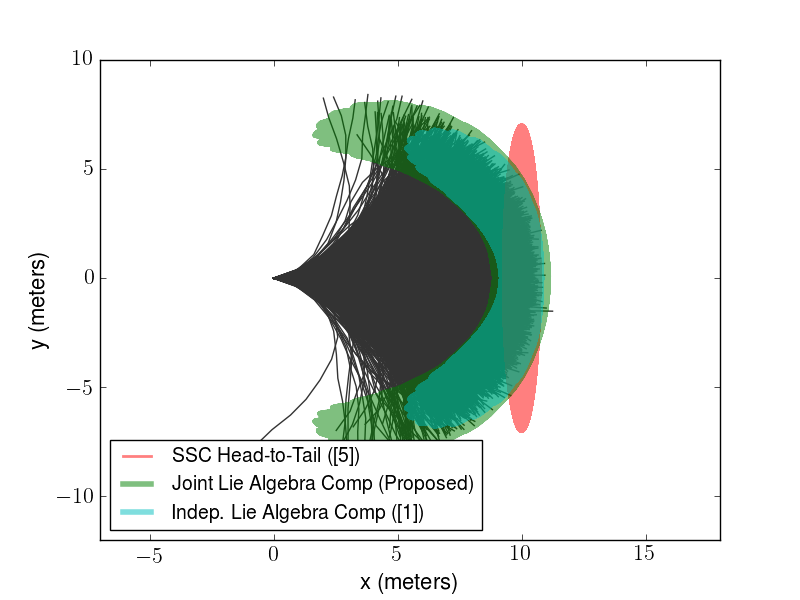
\includegraphics[width=\columnwidth]{figures/10_nodes_sim_correlated.png}
    \caption{
    10000个样本轨迹的绘图,每个轨迹由10个噪声位姿变换组成。95\%可能的不确定性椭圆,通过SSC头到尾(head-to-tail)操作的一阶不确定性传播预测,以红色显示,当考虑相关性和不考虑相关性时,扁平的95\%可能的不确定性位置椭圆,通过李代数位姿组合方法预测,分别用绿色和青色表示。 }
    \label{fig:compose_example}
\end{figure}

虽然在文献 \cite{smith1990a} 中提出的SSC操作和本文提出的基于李代数的方法(以及文献 \cite[(55)]{barfoot2014associating} 中的 $\Sigma_{2nd}$)都是一阶近似方法(就协方差项而言),在李代数空间中刻画旋转不确定性的结果是对位姿不确定性的更精确地刻画。 
这是因为欧拉角参数化是一个图表(chart),并没有覆盖整个流形,而李代数内在地捕获了群结构,可以对任何任意群元素进行建模。此外,由于李代数是一个向量空间~\cite{tapp2016matrix},因此将不确定性建模为高斯分布是方便的,并且定义明确。 

为了证明这一点,我们进行了一个类似于文献\cite{barfoot2014associating}中提出的实验。 
我们生成了一个形式为 $\mathbf{T}_{ab} = \operatorname{exp}(\boldsymbol{\xi}_{ab}^{\wedge}) \bar{\mathbf{T}}_{ab}$ 的 $N$ 个噪声位姿变换序列,其中 
\begin{equation}
    \boldsymbol{\xi}_{ab} \sim \mathcal{N}(\mathbf{0}, \boldsymbol{\Sigma}_{ab}),
\end{equation}
\begin{equation}
    \boldsymbol{\Sigma}_{ab} = \operatorname{diag}([ 0.001\sigma_t, 1e^{-5}\sigma_t, 1e^{-5}, 1e^{-5}, 1e^{-5}, 0.003\sigma_r]),
\end{equation}
并且
\begin{equation}
    \bar{\mathbf{T}}_{ab} = \left[ \begin{array}{cccc}
        1 & 0 & 0 & 1 \\
        0 & 1 & 0 & 0 \\
        0 & 0 & 1 & 0 \\
        0 & 0 & 0 & 1
    \end{array} \right],
\end{equation}
其中 $\sigma_t$ 和 $\sigma_r$ 分别为平移和旋转噪声的缩放参数。 
此外,绘制了每个连续的扰动变量 $\boldsymbol{\xi}_{ab}$,使得它与相关系数 $\rho$ 之前的扰动变量相关。 

然后,我们将这些变换进行端对端组合,并重复这一过程以生成10000个样本轨迹。 
然后,这些蒙特卡洛模拟结果被用来评估SSC头到尾(head-to-tail)操作预测的不确定性,以及本节推导的基于李代数的位姿组合方法,同时考虑了相关和不相关。一个这样的实验的俯视图,$N=10$,$\sigma_t=5$,$\sigma_r=5$,和$\rho=0.4$ 如 \figref{fig:compose_example} 所示。 

正如预期的那样,基于李代数的方法明显优于SSC头到尾(head-to-tail)的方法,因为它考虑了 $\mathrm{SE}(3)$ 的群结构。此外,这很容易看出,如果确实存在正相关,放弃交叉协方差项会导致对真实协方差的近似不足。 
对这个实验更深入的研究在第 \secref{sec:eval:composition} 节中描述。 

在接下来的两节中,我们提供了李代数中的位姿求逆和相对位姿操作的推导,据我们所知,这些推导以前还没有发表过。 


\section{位姿求逆操作}
\label{sec:inverse}

位姿求逆操作对应于参照帧中的更改。 
给定一个不确定的位姿分布 $\mathbf{T}_{ij}$,它代表坐标帧 $j$ 相对于帧 $i$ 的位姿,我们希望找到代表坐标帧 $i$ 相对于帧 $j$ 的位姿求逆 $\mathbf{T}_{ji}$。 
一个位姿求逆的分布可导出如下 \cite{eade2017lie}: 
\begin{align}
    \mathbf{T}_{ji} &= \mathbf{T}_{ij}^{-1} \nonumber\\
    &= \bar{\mathbf{T}}_{ij}^{-1} \operatorname{exp}(- \boldsymbol{\xi}_{ij}^{\wedge}) \label{eq:pose_inverse}\\
    &= \operatorname{exp}((-\mathrm{Ad}_{\bar{\mathbf{T}}_{ij}^{-1}}\boldsymbol{\xi}_{ij})^\wedge) \bar{\mathbf{T}}_{ij}^{-1} \nonumber\\
    &= \operatorname{exp}(\boldsymbol{\xi}'_{ij}) \bar{\mathbf{T}}_{ij}^{-1} \nonumber
\end{align}
其中 $\boldsymbol{\xi}'_{ij}$ 是原始扰动 $\boldsymbol{\xi}_{ij}$ 由 $\bar{\mathbf{T}}_{ij}^{-1}$ 执行负伴随的变换。 %\mgj{This is confusing, previously $\boldsymbol{\xi}'_{ij}$ didn't have the negative sign. It's obviously ok but it's better to keep it simple.}
由于伴随算子的线性,我们可以用均值和协方差表示求逆分布 $\mathbf{T}_{ji}$ 
\begin{align}
    \bar{\mathbf{T}}_{ji} = \bar{\mathbf{T}}_{ij}^{-1}
\end{align}
并且
\begin{align}
    \boldsymbol{\Sigma}_{ji} = \mathrm{Ad}_{\bar{\mathbf{T}}_{ij}^{-1}} \boldsymbol{\Sigma}_{ij} \mathrm{Ad}_{\bar{\mathbf{T}}_{ij}^{-1}}^\top.
\end{align}

\section{寻找联合分布位姿之间的相对变换}
\label{sec:relative_pose}

本节结合前两节的推导,制定了一阶方法,用于刻画相对位姿操作的不确定性,或与第 \ref{sec:SSC:tail-to-tail} 节中描述的SSC尾对尾(tail-to-tail)操作等同的无坐标操作。据我们所知,这是第一次用李代数来刻画不确定性时发表这个操作。 

\subsection{相对位姿操作推导}

\begin{figure}[t]
    \centering
    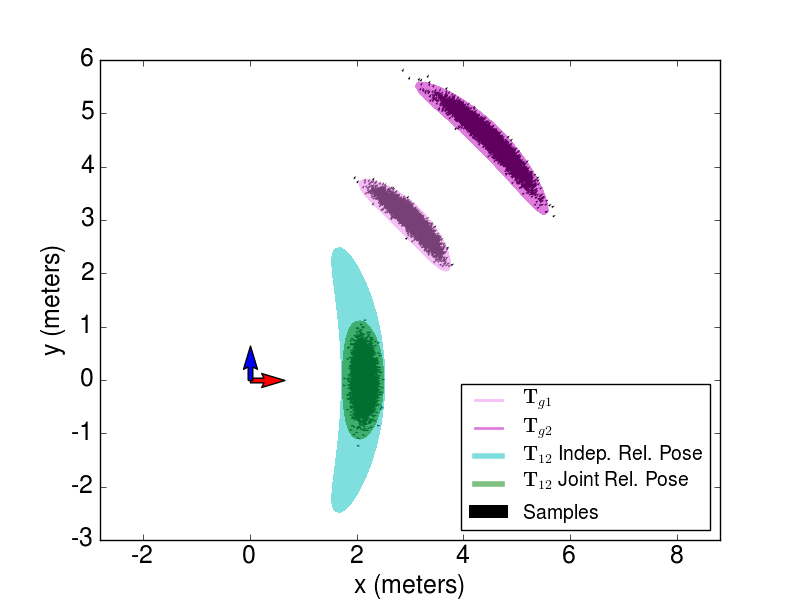
\includegraphics[width=\columnwidth]{figures/between_plot.png}
    \caption{消除方程 \eqref{eq:pose_compound_cov} 和方程 \eqref{eq:relative_pose_cov} 中的相关项可能导致对不确定性的低估/高估。在本例中,我们使用我们提议的方法来估计两个相关位姿 $\mathbf{T}_{g1}$ 和 $\mathbf{T}_{g2}$ 之间的相对位姿 $\mathbf{T}_{12}$。当忽略相关性(方程 \eqref{eq:relative_pose_cov} 不带交叉项)和考虑相关性(方程\eqref{eq:relative_pose_cov} 带上所有项)时,预测95\%可能的不确定性椭圆的扁平视图分别以青色和绿色显示。该图是在 $\alpha=1$ 时绘制的。}
    \label{fig:between}
\end{figure}

\begin{figure}[t]
    \centering
    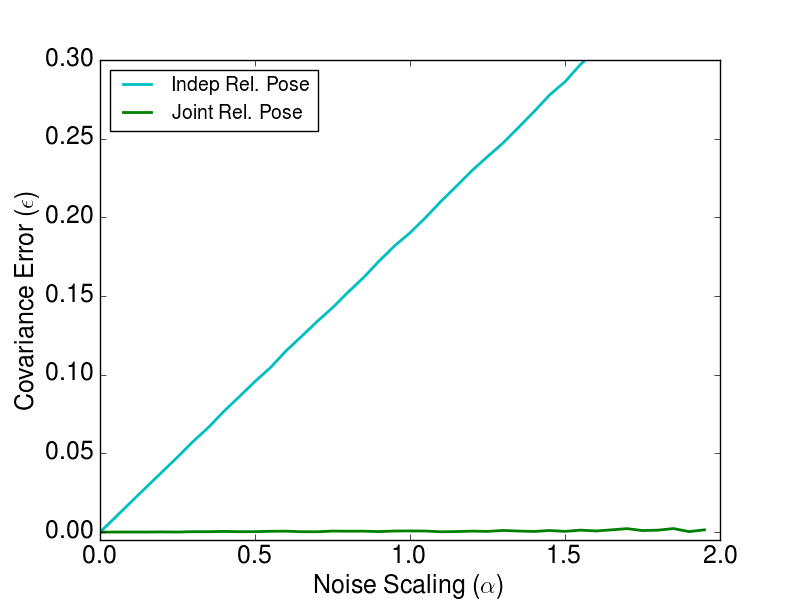
\includegraphics[width=\columnwidth]{figures/between_covariance_error.png}
    \caption{协方差误差比较显示传播不确定性时不忽略相关性的重要性。}
    \label{fig:cov_error}
\end{figure}

给定两个坐标帧相对于一个公共基帧的不确定估计,我们的目的是估计两个姿态之间的相对变换。例如,给定可能相关的不确定变换 $\mathbf{T}_{ij}$ 和 $\mathbf{T}_{ik}$,表示坐标帧 $j$ 和 $k$ 相对于帧 $i$ 的位姿,我们想找到均值 $\bar{\mathbf{T}}_{jk}$ 和协方差 $\boldsymbol{\Sigma}_{jk}$,它们参数化了帧 $k$ 相对于帧 $j$ 的位姿不确定性。 

我们首先假设 $\bar{\mathbf{T}}_{ij}$ 和 $\bar{\mathbf{T}}_{ik}$ 是已知的,相关的扰动 
$\boldsymbol{\xi}_{ij}$ 和 $\boldsymbol{\xi}_{ik}$
在李代数中与已知的协方差联合相关 
\begin{align}
    \boldsymbol{\Sigma} 
    &= 
    \left[ \begin{array}{cc}
        \boldsymbol{\Sigma}_{ij} & ~~~\boldsymbol{\Sigma}_{ij,ik}  \\
        ~~~\boldsymbol{\Sigma}_{ij,ik}^\top & \boldsymbol{\Sigma}_{ik}
    \end{array} \right]. \nonumber
\end{align} 
在标准的群求逆和乘法操作下,必须满足以下条件:
\begin{equation}
    \mathbf{T}_{jk} = \mathbf{T}_{ij}^{-1} \mathbf{T}_{ik}. \label{eq:relative_pose}
\end{equation}
使用方程 \eqref{eq:T_i} 中的随机变量定义扩展方程 \eqref{eq:relative_pose},并在方程 \eqref{eq:pose_inverse} 中推导,其结果是 
\begin{align}
    \operatorname{exp}(\boldsymbol{\xi}_{jk}^\wedge) \bar{\mathbf{T}}_{jk} 
    &= 
    \bar{\mathbf{T}}_{ij}^{-1}
    \operatorname{exp}(-\boldsymbol{\xi}_{ij}^\wedge) 
    \operatorname{exp}(\boldsymbol{\xi}_{ik}^\wedge) \bar{\mathbf{T}}_{ik} \\
    &= 
    \operatorname{exp}((-\mathrm{Ad}_{\bar{\mathbf{T}}_{ij}^{-1}}\boldsymbol{\xi}_{ij})^\wedge) \bar{\mathbf{T}}_{ij}^{-1}
    \operatorname{exp}(\boldsymbol{\xi}_{ik}^\wedge) \bar{\mathbf{T}}_{ik} \nonumber\\
%     &= 
%    \operatorname{exp}((-\mathrm{Ad}_{\bar{\mathbf{T}}_{ij}^{-1}}\boldsymbol{\xi}_{ij})^\wedge)
%    \operatorname{exp}((\mathrm{Ad}_{\bar{\mathbf{T}}_{ij}^{-1}}\boldsymbol{\xi}_{ik})^\wedge)
%    \bar{\mathbf{T}}_{ij}^{-1}
%     \bar{\mathbf{T}}_{ik} \nonumber\\
    &= 
    \operatorname{exp}(\boldsymbol{\xi}_{ij}^{\prime\wedge})
    \operatorname{exp}(\boldsymbol{\xi}_{ik}^{\prime\wedge})
    \bar{\mathbf{T}}_{ij}^{-1}
     \bar{\mathbf{T}}_{ik}, \nonumber     
\end{align}
其中 $\boldsymbol{\xi}_{ij}^\prime = -\mathrm{Ad}_{\bar{\mathbf{T}}_{ij}^{-1}}\boldsymbol{\xi}_{ij}$ 并且 $\boldsymbol{\xi}_{ik}^\prime = \mathrm{Ad}_{\bar{\mathbf{T}}_{ij}^{-1}}\boldsymbol{\xi}_{ik}$。 %\mgj{Again it's confusing and inconsistent, one with negative and one without.}
设
\begin{equation}
    \bar{\mathbf{T}}_{jk} \triangleq \bar{\mathbf{T}}_{ij}^{-1} \bar{\mathbf{T}}_{ik}, \label{eq:relative_pose_mu}
\end{equation}
让我们得到
\begin{equation}
     \operatorname{exp}(\boldsymbol{\xi}_{jk}^\wedge) = \operatorname{exp}(\boldsymbol{\xi}_{ij}^{\prime\wedge})
    \operatorname{exp}(\boldsymbol{\xi}_{ik}^{\prime\wedge}).
\end{equation}
以类似于方程
\eqref{eq:BCH_compound_pose} 的方式扩展BCH公式,并采用方程 \eqref{eq:2nd_order} 中的期望值,得到以下到一阶结果: 
\begin{align}
    E[\xib{jk}\xibt{jk}] \approx &E [ \xip{ij}\xipt{ij} ] + E[\xip{ik}\xipt{ik}] ~+  \label{eq:relative_pose_cov_expectation}\\       
    &+E[\xip{ij}\xipt{ik}] + E[\xip{ik}\xipt{ij}]. \nonumber
\end{align} 
在方程 \eqref{eq:relative_pose_cov_expectation} 中评估期望,其结果是 
\begin{align}
    \boldsymbol{\Sigma}_{jk} \approx
    &\mathrm{Ad}_{\bar{\mathbf{T}}_{ij}^{-1}} \boldsymbol{\Sigma}_{ij} \mathrm{Ad}_{\bar{\mathbf{T}}_{ij}^{-1}}^\top +
    \mathrm{Ad}_{\bar{\mathbf{T}}_{ij}^{-1}} \boldsymbol{\Sigma}_{ik} \mathrm{Ad}_{\bar{\mathbf{T}}_{ij}^{-1}}^\top - \label{eq:relative_pose_cov}\\
    &+\mathrm{Ad}_{\bar{\mathbf{T}}_{ij}^{-1}} \boldsymbol{\Sigma}_{ij,ik} \mathrm{Ad}_{\bar{\mathbf{T}}_{ij}^{-1}}^\top -
    \mathrm{Ad}_{\bar{\mathbf{T}}_{ij}^{-1}} \boldsymbol{\Sigma}_{ij,ik}^\top \mathrm{Ad}_{\bar{\mathbf{T}}_{ij}^{-1}}^\top. \nonumber
\end{align}

因此,不确定性可以通过方程
\eqref{eq:relative_pose_mu} 和方程 \eqref{eq:relative_pose_cov} 的相对位姿函数来进行传播。在前面三节中得出的不确定性传播方法总结在 \figref{fig:summary} 中提供。 

\subsection{忽略相关性导致不一致}

忽略相关扰动变量的相关性会导致不确定性的低估/高估,这取决于相关性是正还是负,以及所执行的操作是位姿组合还是相对位姿估计。 
\figref{fig:between} 和 \figref{fig:cov_error} 显示了一个关于具有正相关的相对位姿的例子。 

为了创建这些图。我们生成了 $M=10000$ 的两组不确定位姿 $\mathbf{T}^m_{g1}=\operatorname{exp}(\boldsymbol{\xi}_{g1}^{m\wedge}) \bar{\mathbf{T}}_{g1}$  和 $\mathbf{T}_{g2}=\operatorname{exp}(\boldsymbol{\xi}_{g2}^{m\wedge}) \bar{\mathbf{T}}_{g2}$,其均值为 
\begin{equation}
    \bar{\mathbf{T}}_{g1} = \left[ \begin{array}{cccc}
        0.707107 & -0.707107  & 0      & 3 \\
        0.707107 &  0.707107  & 0      & 3 \\
       -0        &  0         & 1      & 0 \\
        0        &  0         & 0      & 1
    \end{array} \right]
\end{equation}  
并且
\begin{equation}
    \bar{\mathbf{T}}_{g2} = \left[ \begin{array}{cccc}
        0.707107 & -0.707107  & 0      & 4.5 \\
        0.707107 &  0.707107  & 0      & 4.5 \\
       -0        &  0         & 1      & 0 \\
        0        &  0         & 0      & 1
    \end{array} \right],
\end{equation}
在扰动变量($\boldsymbol{\xi}^m_{g1}$) 和 ($\boldsymbol{\xi}^m_{g2}$) 在李代数中是联合相关的假设下,边际协方差矩阵为 
\begin{align}
    \boldsymbol{\Sigma}_{g1} &= \boldsymbol{\Sigma}_{g2}  \\
    &= \alpha \cdot \operatorname{diag}([0.005, 0.005, 1e-5, 1e-5, 1e-5, 0.006]),  \nonumber
\end{align}
并且交叉协方差为
\begin{equation}
    \boldsymbol{\Sigma}_{g1,g2} = \alpha \cdot \operatorname{diag}([0.0005, 0.0005, 0, 0, 0, 0.005]),
\end{equation}
其中 $\alpha$ 是缩放参数。 
然后,我们使用本节中介绍的相对位姿操作来估计 $\mathbf{T}_{12}$,同时考虑和不考虑不确定性的情况。 


在 \figref{fig:cov_error} 中,在以下协方差误差度量下,对于增加与蒙特卡罗模拟有关的 $\alpha$ 的值,我们评估了估计协方差误差 
\begin{equation}
    \epsilon \triangleq \sqrt{\operatorname{tr}\left( (\boldsymbol{\Sigma} - \boldsymbol{\Sigma}_{mc})^\top (\boldsymbol{\Sigma} - \boldsymbol{\Sigma}_{mc}) \right)}, \label{eq:cov_error}
\end{equation}
其中 
\begin{equation}
\boldsymbol{\Sigma}_{mc} = \frac{1}{M}\sum_{m=1}^M \boldsymbol{\xi}_m \boldsymbol{\xi}_m^{\top},\label{eq:sample_mc_cov}
\end{equation}
具有 
\begin{equation}
\mathbf{T}_m = (\operatorname{exp}(\boldsymbol{\xi}_{g1}^{m\wedge})\bar{\mathbf{T}}_{g1})^{-1}\operatorname{exp}(\boldsymbol{\xi}_{g2}^{m\wedge})\bar{\mathbf{T}}_{g2} \label{eq:sample_mc_mean}
\end{equation}
和 
\begin{equation}
\boldsymbol{\xi}_m = \operatorname{log}(\mathbf{T}_m \bar{\mathbf{T}}_{12}^{-1})^\vee.   
\label{eq:sample_mc_xi}
\end{equation}
\figref{fig:compose_example},\figref{fig:between},和 \figref{fig:cov_error} 表明,忽略相关性会导致不确定性的估计不一致。

\section{转换为基于李代数的表示}
\label{sec:conversion}

尽管李代数中的不确定性刻画比基于坐标的方法更精确,但在某些情况下,现有的估计算法可能会以另一种参数化方式输出位姿估计。 
本节介绍如何从现有参数化,如SSC多元变量高斯表示法(定义在方程 \eqref{eq:SSC_rep} 和方程 \eqref{eq:SSC_joint_rep} 中),转换为提议的表示法,以及如何从 MLE 的解中,如iSAM \cite{kaess2008isam} 或 g2o \cite{kummerle2011g2o},直接提取联合相关位姿集合的均值和协方差。  

\subsection{从基于坐标的表示法转换}

\begin{figure}[t]
    \centering
    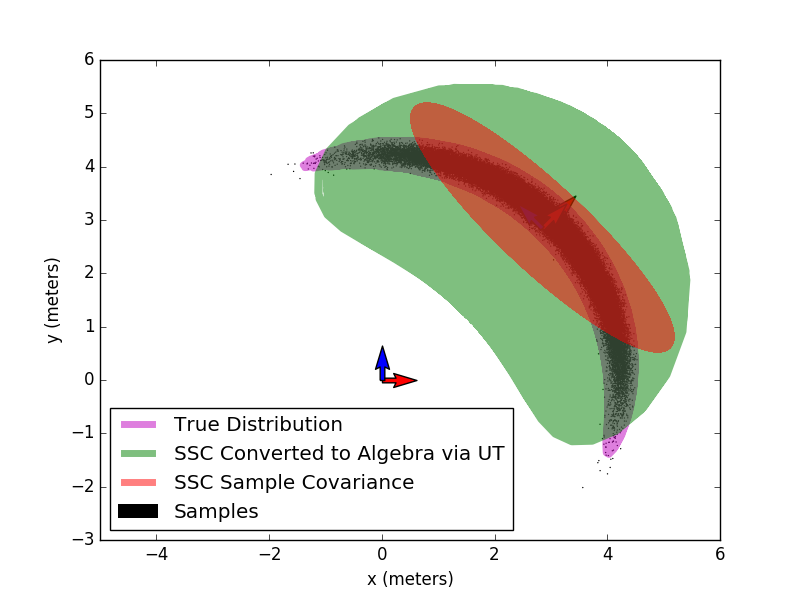
\includegraphics[width=\columnwidth]{figures/UT-Conv-SSC.png}
    \caption{无味变换 (UT) \cite{julier2002scaled} 可用于从现有的基于坐标的表示法,如 SSC 方程 \eqref{eq:SSC_rep} (以红色显示) 转换到基于李代数的表示法 (以绿色显示)。然而,首先使用SSC表示法会导致信息丢失,并且生成的表示 (以绿色显示) 过于接近真实的底层分布 (以粉色显示)。所有不确定性界线显示的是95\%可能的椭圆。}
    \label{fig:ut_conversion}
\end{figure}

假设给定一个均值参数向量 $\hat{\mathbf{x}}$ 和相关协方差 $\hat{\boldsymbol{\Sigma}}$,如方程 \eqref{eq:SSC_joint_rep} 中所定义,以应用我们提议的传播方法,我们必须首先将 $\hat{\mathbf{x}}$ 和 $\hat{\boldsymbol{\Sigma}}$ 变换成我们所提议的表示,使得相关变换的方法通过 $\bar{\mathbf{T}}_{1:n}$ 在群空间中表示,并且扰动被表示为多元高斯随机变量,$\boldsymbol{\xi}_{1:n}$,其协方差 $\boldsymbol{\Sigma}_{1:n}$,在相关的李代数中定义在方程 \eqref{eq:lie_joint_rep_cov} 和方程 \eqref{eq:lie_joint_rep_means} 中。 
从基于坐标的不确定性刻画方法转换为李代数表示法是一种非线性操作。 
因此,与一阶线性化方法相比,无味变换 \cite{julier2002scaled} 是在表示法之间转换的更好选择。 

无味变换是由 \citet{julier1997new} 于1997年首次提出的,它采用在一个空间中定义的输入高斯分布和一个非线性函数,该函数将输入空间映射到输出空间,并为变换后的分布找到高斯近似值。这是通过使用输入均值和协方差来创建一个有 $K = 2m + 1$ 个sigma点的确定性集合 $\mathcal{X}_{1:K}$,其中 $m$ 是输入空间的维数。然后将这些sigma点通过非线性函数,并使用加权均值和样本协方差来找到输出分布的高斯近似值。 

假设我们有一个函数 $f : \mathbb{R}^d \mapsto \mathcal{G}$,它从一个参数向量 $\mathbf{x}_i$ 映射到李群的一个元素 $\mathcal{G}$,我们可以定义一个函数 $\ell_i$,它接受一个扰动参数向量 $\tilde{\mathbf{x}}_i$,在幺元上以其为中心,并将其变换到李代数空间,如下所示: 
\begin{equation}
    \ell_i(\tilde{\mathbf{x}}_i) = \operatorname{log}( f(\tilde{\mathbf{x}}_i) \cdot f(\hat{\mathbf{x}}_i)^{-1} ),
\end{equation}
其中 $\hat{\mathbf{x}}_i$ 是与 $\tilde{\mathbf{x}}_i$ 相关联的均值参数向量。 

然后,我们可以使用标准的无味变换 \cite[(12)]{julier1997new} 来从 $\hat{\mathbf{x}}$ 和 $\hat{\boldsymbol{\Sigma}}$ 生成 $2nd + 1$ 个sigma点的集合 $\mathcal{X}_{1:K}$,其中,$n$ 是已建模的李群元素的数量。 
之后,可获得联合相关位姿的预测李群表示,如下所示: 
\begin{equation}
    \bar{\mathbf{T}}_i = f(\hat{\mathbf{x}}_i)
\end{equation}
\begin{equation}
    \boldsymbol{\Sigma}_{1:n} = \sum_{k=1}^K \mathcal{W}_k \ell(\mathcal{X}_k) \ell(\mathcal{X}_k)^\top,
\end{equation}
其中 $\ell$ 是 $\ell_i$ 的向量化版本,$\mathcal{W}_k$ 是来自文献 \cite[(12)]{julier1997new} 的标准权重。 
\figref{fig:ut_conversion} 显示此过程的结果。

尽管在许多情况下,使用无迹变换可能是最好的方法,但使用基于坐标的表示(即使作为中间表示)确实会导致一些信息损失。 
从先验估计解中提取不确定性时,如果我们能直接表示框架中的不确定性,就可以避免这种信息损失。 

\subsection{从MLE解中提取位姿不确定性}
\label{sec:convert:cov_extraction}

最先进的位姿图SLAM求解器通过估计机器人位姿集合来找到问题的解,从而最大化观测测量的可能性 \cite{dellaert2006a, kaess2008isam, kaess2011isam2, rosen2016sesync, jmangelson-2019a}。 
传统的迭代非线性求解器 \cite{dellaert2006a, kaess2008isam, kaess2011isam2, kummerle2011g2o} 通过建立一个测量Jacobian矩阵,$A$,其列对应于参数向量 $\mathbf{x}$ 的元素,并且其块行对应于加权,测量残差误差函数,使得预测测量值和实际测量值之间的误差最小化。 
在每次迭代中,该测量Jacobian矩阵用来形成以下形式的线性最小二乘问题: 
\begin{equation}
    \hat{\mathbf{x}} = \underset{\mathbf{x}}{\operatorname{argmin}} \lVert A \mathbf{x} - \mathbf{b} \rVert^2,
\end{equation}
其中 $\mathbf{b}$ 是以下推导中不需要的测量向量。 
该算法交替地解决线性最小二乘优化问题以及围绕着 $\hat{\mathbf{x}}$ 重新线性化 $A$ 矩阵直至收敛 \cite{dellaert2006a, kaess2008isam}。 
提供全局最优性保证的算法,如在文献 \cite{rosen2016sesync} 和文献 \cite{jmangelson-2019a} 中描述的算法,对问题的描述略有不同,但一旦得到一个解,仍然可以通过围绕当前的解,线性化损失来形成矩阵 $A$。

在获得一个解之后,通过使用 $A$ 形成信息矩阵 $\mathcal{I}= A^\top A$ 并使用其Cholesky因子化的非零元素 $\mathcal{I}= R^\top R$ 来计算边际协方差 $\hat{\boldsymbol{\Sigma}}$ 的必要元素,可以找到该解的不确定性的估计,如文献 \cite{kaess2009covariance} 中所述。 
相对于 $\hat{\mathbf{x}}$ ,提取这个协方差的诀窍是确保用于形成 $\mathcal{I}$ 的Jacobian矩阵 $A$ 是相对于 $\boldsymbol{\xi}_{1:n}$ 评估的,而不是相对于 $\hat{\mathbf{x}}$。 
这可以通过数值评估Jacobian矩阵以及围绕着 $\mathbf{0}$ 的扰动 $\boldsymbol{\xi}_{1:n}$,并通过指数函数将扰动传播到线性化点,而不是直接扰动 $\hat{\mathbf{x}}$ 的参数。
这样做可以直接提取 $\boldsymbol{\Sigma}_{1:n}$,并提高精度,因为 $\boldsymbol{\xi}_{1:n}$ 位于向量空间中,而 $\hat{\mathbf{x}}$ 不在。 

\section{评估}
\label{sec:eval}

本节通过两个实验来评估所提议的不确定度刻画方法。 
首先,对第 \secref{sec:pose_composition:comparison} 节中介绍的实验进行参数扫描。 
其次,从位姿图SLAM算法的结果中提取协方差信息,并将预测的相对位姿协方差与蒙特卡洛获得的样本协方差进行比较。 

\subsection{联合相关里程计}
\label{sec:eval:composition}

\begin{figure}[t]
    \centering
    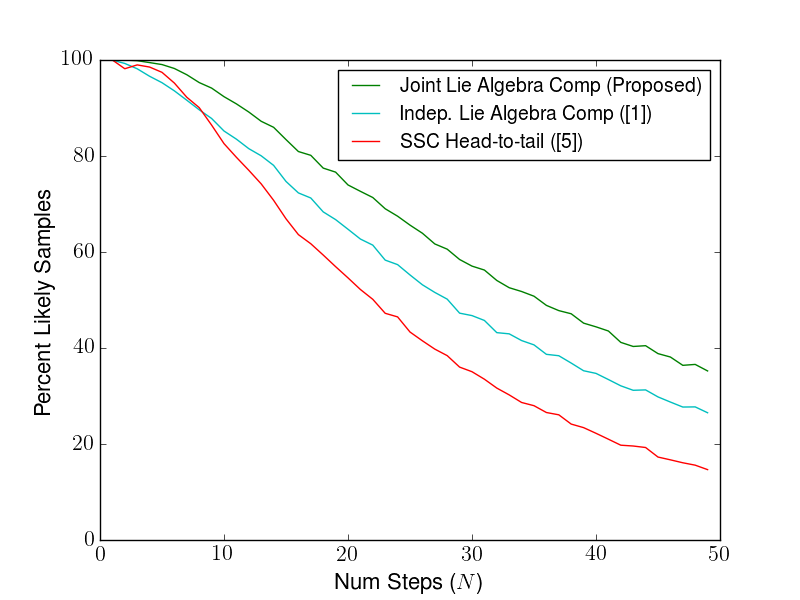
\includegraphics[width=\columnwidth]{figures/compose_num_steps.png}
    \caption{最终样本在99.9\%可能的协方差椭圆内的百分比,作为轨迹序列中位姿数量的函数。所有方法都会随着位姿数量的增加而下降,但是我们提出的方法始终是最精确的。}
    \label{fig:compose_num_steps}
\end{figure}
\begin{figure}[t]
    \centering
    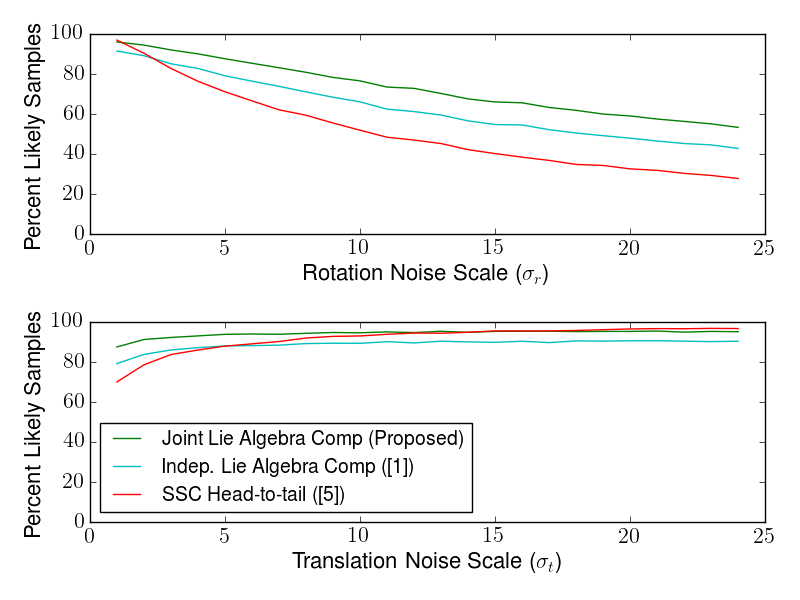
\includegraphics[width=\columnwidth]{figures/compose_noise.png}
    \caption{作为旋转和平移噪声函数,最终样本百分比在99.9\%可能的协方差椭圆内。对于旋转噪声扫描,平移噪声保持不变,在 $\sigma_t=3$ 处,对于平移噪声扫描,旋转噪声保持不变,在 $\sigma_r=3$ 处。注意,旋转噪声的增加会产生最大的负面效应。}
    \label{fig:compose_noise}
\end{figure}

我们提出的不确定性刻画方法的确切精度取决于各种参数,包括端到端位姿组合数量以及旋转和平移的噪声。 
我们根据在 \secref{sec:pose_composition:comparison} 节中介绍的实验,通过对每个参数执行参数扫描来探索这种依赖性。 

%\begin{figure*}[!t]%
%    \centering%
%    \subfloat[Pose Pair Correlation - X\label{fig:x_corr_50}]{%
%       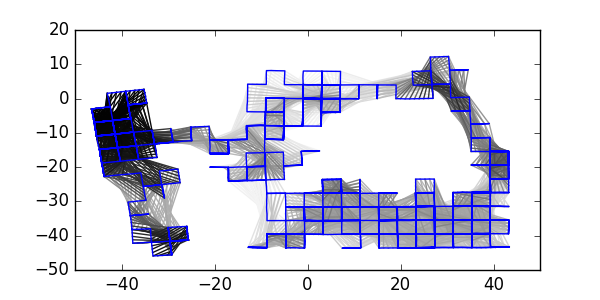
\includegraphics[width=0.33\textwidth,trim={1cm 0 1cm 0},clip]{figures/pose_pair_corr_x_50.png}
%    }
%    \subfloat[Pose Pair Correlation - Y\label{fig:y_corr_50}]{%
%       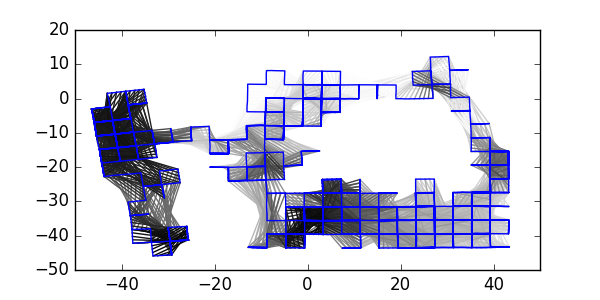
\includegraphics[width=0.33\textwidth,trim={1cm 0 1cm 0},clip]{figures/pose_pair_corr_y_50.png}
%    }
%    \subfloat[Pose Pair Correlation - Heading\label{fig:t_corr_50}]{%
%       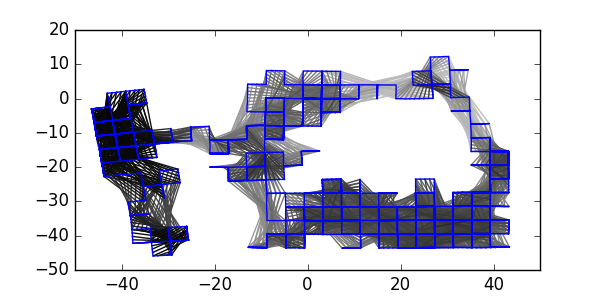
\includegraphics[width=0.33\textwidth,trim={1cm 0 1cm 0},clip]{figures/pose_pair_corr_t_50.png}
%    }
%    \hfill
%    \subfloat[Joint Relative Pose Cov. Error\label{fig:joint_error_50}]{%
%       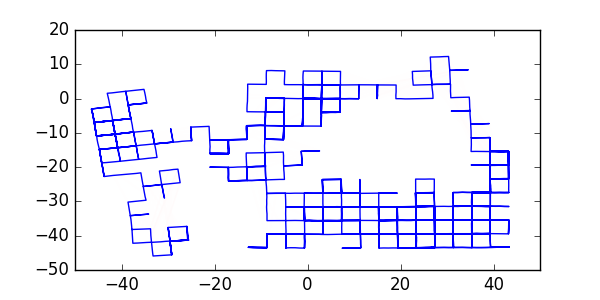
\includegraphics[width=0.45\textwidth,trim={1cm 0 1cm 0},clip]{figures/joint_relative_pose_cov_error_50.png}
%    }
%    \subfloat[Indep. Relative Pose Cov. Error\label{fig:indep_error_50}]{%
%       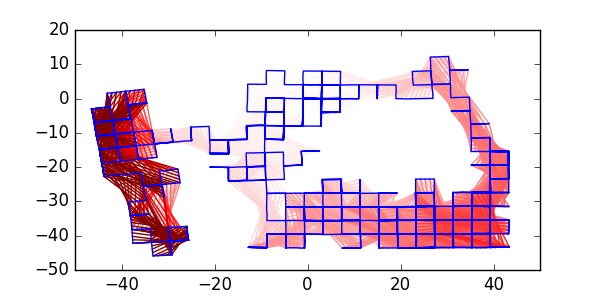
\includegraphics[width=0.45\textwidth,trim={1cm 0 1cm 0},clip]{figures/indep_relative_pose_cov_error_50.png}
%    }\hfill
%  \caption{A visualization of the correlation and covariance error for 3450 pose pairs with an offset of 50 nodes extracted from a solution of the Manhattan3500 dataset \cite{olson2006fast}. \subref{fig:x_corr_50}, \subref{fig:y_corr_50}, and \subref{fig:t_corr_50} show the relative poses colored by the correlation coefficient of the $x$, $y$, and $\theta$ dimensions respectively. White corresponds to a correlation coefficient of 0 and black to a coefficient of 1. \subref{fig:joint_error_50} and \subref{fig:indep_error_50} show the covariance error with respect to Monte Carlo for relative pose estimation in the Lie algebra when correlation is and is not taken into account. Dark red corresponds to a covariance error of at least 2 standard deviations above the mean (with respect to independent relative pose extraction), while white corresponds to a covariance error of 0.}
%  \label{fig:slam_rp_error_50}
%\end{figure*}

\begin{figure*}[!t]%
    \centering%
    \subfloat[位姿对的相关性 - X\label{fig:x_corr_50}]{%
       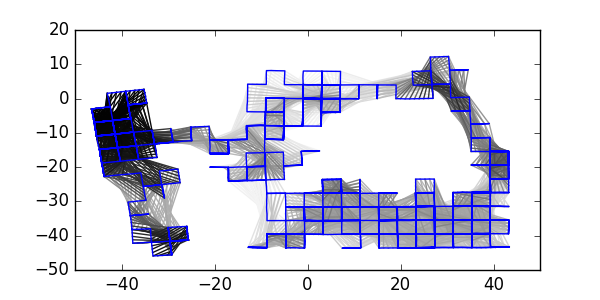
\includegraphics[width=0.33\textwidth,trim={1cm 0 1cm 0},clip]{figures/pose_pair_corr_x_50.png}
    }
    \subfloat[位姿对的相关性 - Y\label{fig:y_corr_50}]{%
       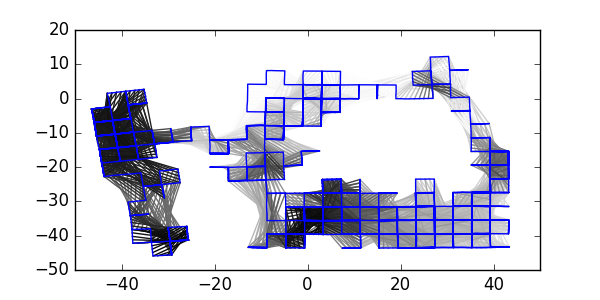
\includegraphics[width=0.33\textwidth,trim={1cm 0 1cm 0},clip]{figures/pose_pair_corr_y_50.png}
    }
    \subfloat[位姿对的相关性 - 航向(Heading)\label{fig:t_corr_50}]{%
       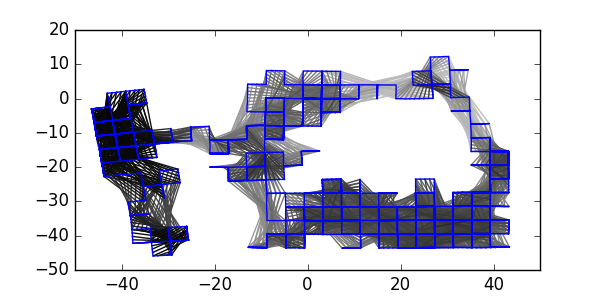
\includegraphics[width=0.33\textwidth,trim={1cm 0 1cm 0},clip]{figures/pose_pair_corr_t_50.png}
    }
    \hfill
    \subfloat[所提议的李代数相对位姿协方差误差\label{fig:joint_error_50}]{%
       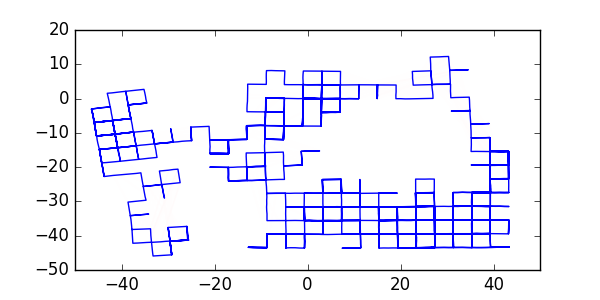
\includegraphics[width=0.4\textwidth,trim={1cm 0 1cm 0},clip]{figures/joint_relative_pose_cov_error_50.png}
    }
    \subfloat[所提议的李代数相对位姿协方差误差(忽略相关性)\label{fig:indep_error_50}]{%
       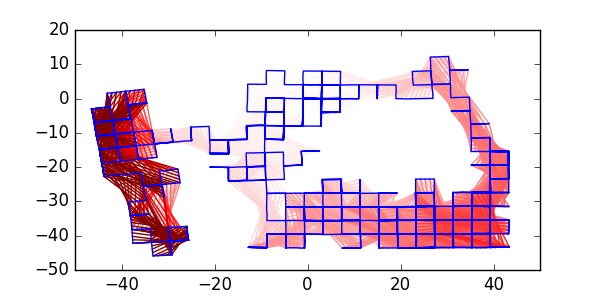
\includegraphics[width=0.4\textwidth,trim={1cm 0 1cm 0},clip]{figures/indep_relative_pose_cov_error_50.png}
    }\hfill
    \subfloat[所提议的李代数相对位姿归一化协方差误差\label{fig:norm_joint_error_50}]{%
       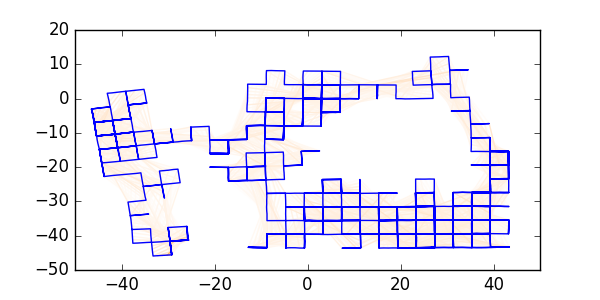
\includegraphics[width=0.4\textwidth,trim={1cm 0 1cm 0},clip]{figures/norm_joint_relative_pose_cov_error_50.png}
    }
    \subfloat[SSC 相对位姿归一化协方差误差\label{fig:norm_ssc_error_50}]{%
       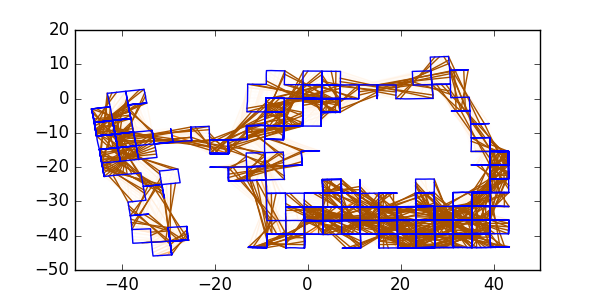
\includegraphics[width=0.4\textwidth,trim={1cm 0 1cm 0},clip]{figures/norm_ssc_relative_pose_cov_error_50.png}
    }\hfill
    \caption{从 Manhattan3500 数据集合 \cite{olson2006fast} 的解中提取的偏移量为50个节点的3450个位姿对的相关性和协方差误差的可视化图。\protect\subref{fig:x_corr_50}、\protect\subref{fig:y_corr_50} 和 \protect\subref{fig:t_corr_50} 分别显示了以 $x$、$y$ 和 $\theta$ 维度的相关系数为颜色的相对位姿。白色对应于相关系数为$0$,黑色对应于系数为$1$。\protect\subref{fig:joint_error_50} 和 \protect\subref{fig:indep_error_50} 显示了,当相关性被考虑和不被考虑时,在李代数中的相对位姿估计相对于蒙特卡罗的协方差误差。暗红色对应于高于平均值至少$2$个标准偏差的协方差误差(相对于忽略相关性时),而白色对应于$0$的协方差误差。\protect\subref{fig:norm_joint_error_50} 和 \protect\subref{fig:norm_ssc_error_50} 显示了所提议的方法和SSC \cite{smith1990a} 相对于蒙特卡罗的归一化协方差误差。在这种情况下,深橙色对应于高于平均值以上至少$2$个标准偏差的协方差误差(相对于SSC相对位姿提取),而白色对应于$0$的协方差误差。}
    \label{fig:slam_rp_error_50}
\end{figure*}




我们首先改变轨迹中位姿的数量($N$),并将两个噪声规模参数固定在 $\sigma_t = \sigma_r = 3$。 
其结果显示在 \figref{fig:compose_num_steps} 中。 
随着步数的增加,最终估计的精度会下降,这是因为每种方法都只刻画一阶不确定性,损失的高阶信息会随着位姿数量的增加而增加。 

\begin{table}[t!]
  \addtolength{\tabcolsep}{-5pt}
  \centering
  \caption{从 Manhattan3500 数据集合 \cite{olson2006fast} 的解中提取的总共44425个位姿对,其中位姿偏移范围为5到500个节点,在考虑和忽略相关性时,所提议的李代数相对位姿估计的协方差误差统计摘要。}
  \scalebox{0.88}{  
  \begin{tabular}{lcc}
    \toprule
    Method & Covariance Error Mean & ~~Covariance Error Std. Dev. \\
    \midrule
    Proposed Lie algebra Rel. Pose &  0.00675104 $\pm~ 2.2e^{-4}$ &  0.0461455\\ %\hline
    Proposed (Ignoring Correlation) & 2.05667 $\pm~ 1.0e^{-2}$ & 2.12371 \\ %\hline    
    \bottomrule
  \end{tabular}
}
%\vspace{-0.6cm}
  \label{table:cov_error}
\end{table}


对于噪声参数实验,我们依次改变噪声规模参数 $\sigma_r$ 和 $\sigma_t$,同时保持位姿数量固定在 $N=10$,并且非变化噪声参数固定在 $3$。 
其结果显示在 \figref{fig:compose_noise} 中。 
旋转噪声的影响更为显著,这同样是因为损失了高阶信息(不论是在BCH公式的高阶项上还是通过SSC的线性化)。 
除了在旋转噪声很低和平移噪声很高的情况下,这两种李群方法始终都优于SSC方法。 
这是因为当旋转误差非常低时,变换的非线性几乎可以忽略不计,并且因为增加的平移误差导致协方差椭圆增加到包含最终机器人位置的点。 
此外,李代数中的联合组合方法始终比忽略相关性时更精确。 
对于所有三个参数扫描,诱导相关性固定在 $\rho=0.4$。 

\subsection{从SLAM的解中提取相对位姿}
\label{sec:eval:relative}

\begin{table}[t!]
  \addtolength{\tabcolsep}{-5pt}
  \centering
  \caption{从 Manhattan3500 数据集合 \cite{olson2006fast} 的解中提取的总共44425个位姿对,对于所提议的方法和 SSC \cite{smith1990a} 的相对位姿估计的标准化协方差误差统计摘要,位姿偏移范围为5到500个节点。}
  \scalebox{0.88}{  
  \begin{tabular}{lcc}
    \toprule
    Method & Normalized Cov. Error Mean & ~~Normalized Cov. Error Std. Dev. \\
    \midrule
    Proposed Rel. Pose &  0.0493121 $\pm~ 1.7e^{-4}$ & 0.0353072\\ %\hline
    SSC Tail-to-Tail & 0.28778 $\pm~ 2.0e^{-3}$ & 0.411625 \\ %\hline    
    \bottomrule
  \end{tabular}
}
%\vspace{-0.6cm}
  \label{table:norm_cov_error}
\end{table}


%\begin{figure*}[!t]%
%    \centering%
%    \subfloat[Pose Pair Correlation - X\label{fig:x_corr_5}]{%
%       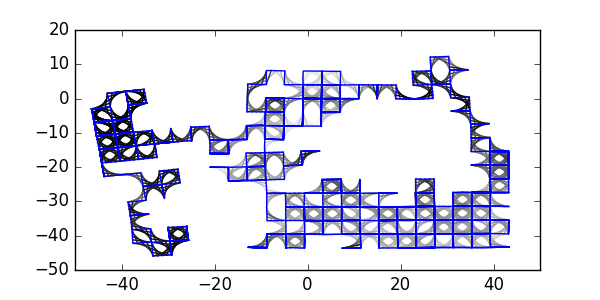
\includegraphics[width=0.33\textwidth,trim={1cm 0 1cm 0},clip]{figures/pose_pair_corr_x_5.png}
%    }
%    \subfloat[Pose Pair Correlation - Y\label{fig:y_corr_5}]{%
%       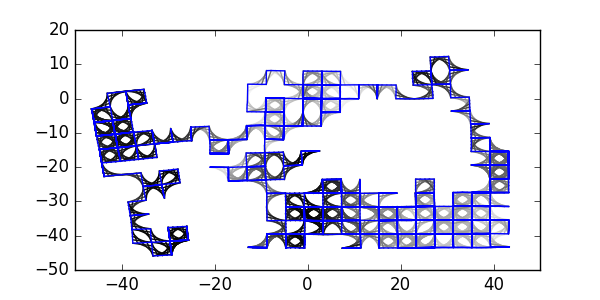
\includegraphics[width=0.33\textwidth,trim={1cm 0 1cm 0},clip]{figures/pose_pair_corr_y_5.png}
%    }
%    \subfloat[Pose Pair Correlation - Heading\label{fig:t_corr_5}]{%
%       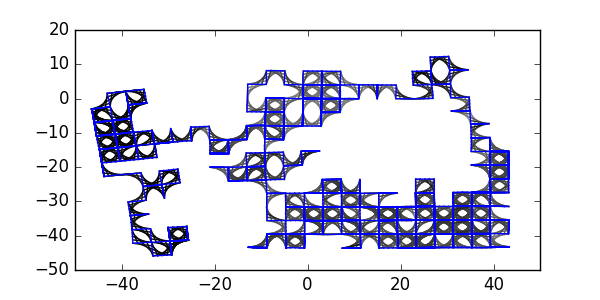
\includegraphics[width=0.33\textwidth,trim={1cm 0 1cm 0},clip]{figures/pose_pair_corr_t_5.png}
%    }
%    \hfill
%    \subfloat[Proposed Lie Algebra Relative Pose Cov. Error\label{fig:joint_error_5}]{%
%       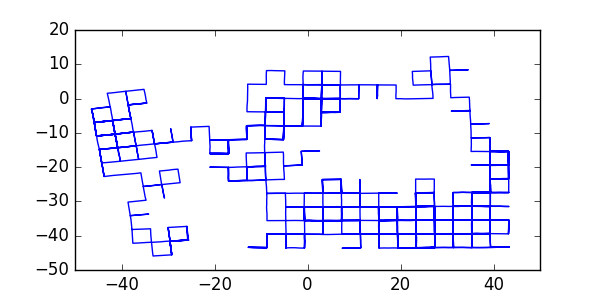
\includegraphics[width=0.39\textwidth,trim={1cm 0 1cm 0},clip]{figures/joint_relative_pose_cov_error_5.png}
%    }
%    \subfloat[Proposed Relative Pose Cov. Error (Ignoring Correlation)\label{fig:indep_error_5}]{%
%       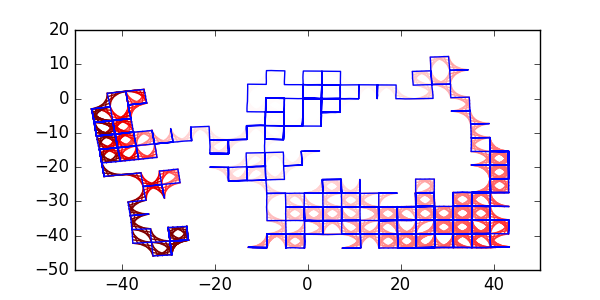
\includegraphics[width=0.39\textwidth,trim={1cm 0 1cm 0},clip]{figures/indep_relative_pose_cov_error_5.png}
%    }\hfill
%        \subfloat[Proposed Lie Algebra Relative Pose Normalized Cov. Error\label{fig:norm_joint_error_5}]{%
%       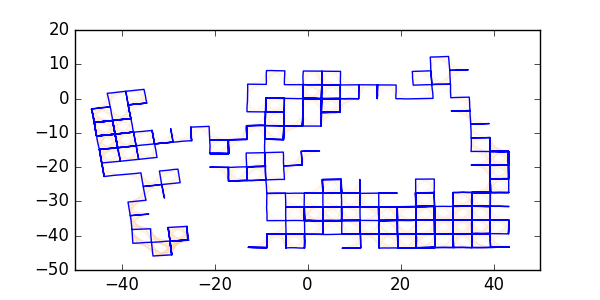
\includegraphics[width=0.39\textwidth,trim={1cm 0 1cm 0},clip]{figures/norm_joint_relative_pose_cov_error_5.png}
%    }
%    \subfloat[SSC Relative Pose Normalized Cov. Error\label{fig:norm_ssc_error_5}]{%
%       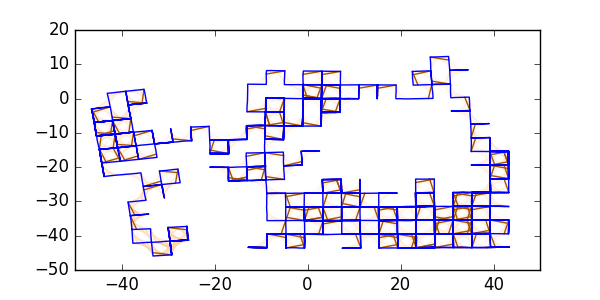
\includegraphics[width=0.39\textwidth,trim={1cm 0 1cm 0},clip]{figures/norm_ssc_relative_pose_cov_error_5.png}
%    }\hfill
%  \caption{A visualization of the correlation and covariance error for 3495 pose pairs with an offset of 5 nodes extracted from a solution of the Manhattan3500 dataset \cite{olson2006fast}. The %color schemes match those of \figref{fig:slam_rp_error_50}.}
%  \label{fig:slam_rp_error_5}
%\end{figure*}

\begin{figure*}[!t]%
    \centering%
    \subfloat[位姿对的相关性 - X\label{fig:x_corr_10}]{%
       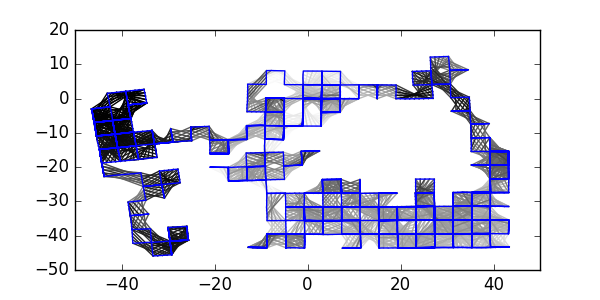
\includegraphics[width=0.33\textwidth,trim={1cm 0 1cm 0},clip]{figures/pose_pair_corr_x_10.png}
    }
    \subfloat[位姿对的相关性 - Y\label{fig:y_corr_10}]{%
       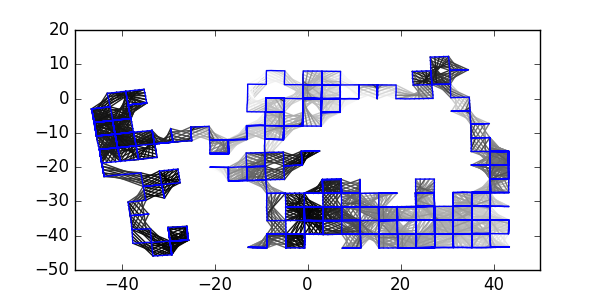
\includegraphics[width=0.33\textwidth,trim={1cm 0 1cm 0},clip]{figures/pose_pair_corr_y_10.png}
    }
    \subfloat[位姿对的相关性 - 航向(Heading)\label{fig:t_corr_10}]{%
       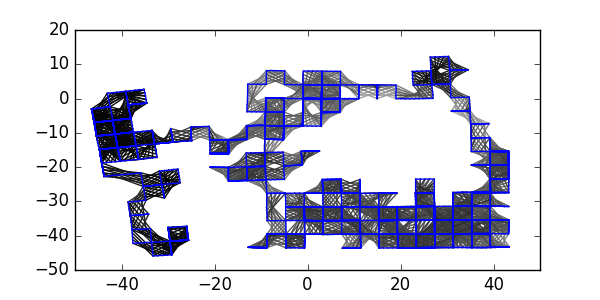
\includegraphics[width=0.33\textwidth,trim={1cm 0 1cm 0},clip]{figures/pose_pair_corr_t_10.png}
    }
    \hfill
    \subfloat[所提议的李代数相对位姿协方差误差\label{fig:joint_error_10}]{%
       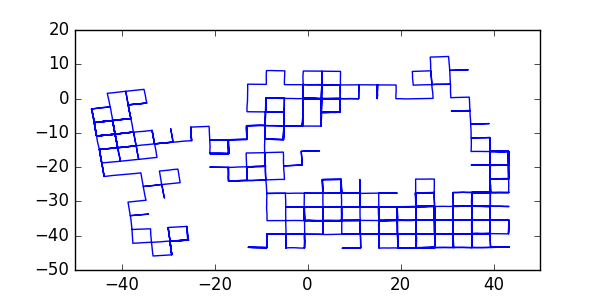
\includegraphics[width=0.39\textwidth,trim={1cm 0 1cm 0},clip]{figures/joint_relative_pose_cov_error_10.png}
    }
    \subfloat[所提议的李代数相对位姿协方差误差(忽略相关性)\label{fig:indep_error_10}]{%
       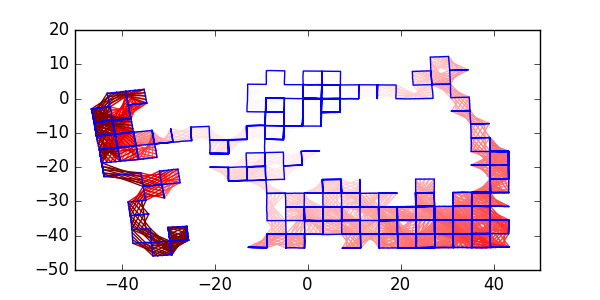
\includegraphics[width=0.39\textwidth,trim={1cm 0 1cm 0},clip]{figures/indep_relative_pose_cov_error_10.png}
    }\hfill
        \subfloat[所提议的李代数相对位姿归一化协方差误差\label{fig:norm_joint_error_10}]{%
       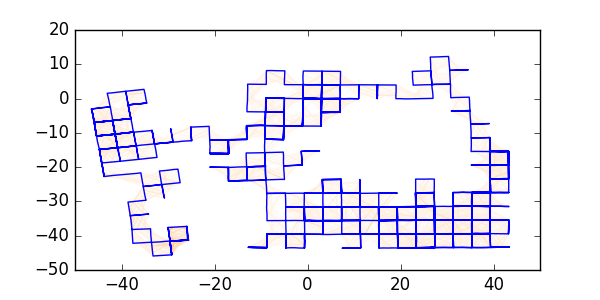
\includegraphics[width=0.39\textwidth,trim={1cm 0 1cm 0},clip]{figures/norm_joint_relative_pose_cov_error_10.png}
    }
    \subfloat[SSC 相对位姿归一化协方差误差\label{fig:norm_ssc_error_10}]{%
       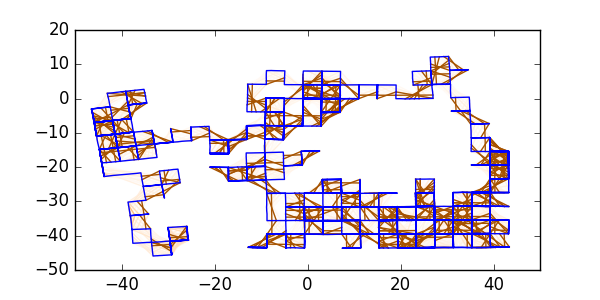
\includegraphics[width=0.39\textwidth,trim={1cm 0 1cm 0},clip]{figures/norm_ssc_relative_pose_cov_error_10.png}
    }\hfill
  \caption{从 Manhattan3500 数据集合 \cite{olson2006fast} 的解中提取的偏移量为10个节点的3490个位姿对的相关性和协方差误差的可视化图。配色方案与 \figref{fig:slam_rp_error_50} 的配色方案相匹配。}
  \label{fig:slam_rp_error_10}
\end{figure*}

\begin{figure*}[!t]%
    \centering%
    \subfloat[位姿对的相关性 - X\label{fig:x_corr_100}]{%
       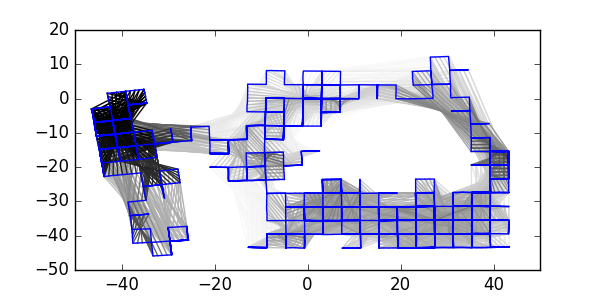
\includegraphics[width=0.33\textwidth,trim={1cm 0 1cm 0},clip]{figures/pose_pair_corr_x_100.png}
    }
    \subfloat[位姿对的相关性 - Y\label{fig:y_corr_100}]{%
       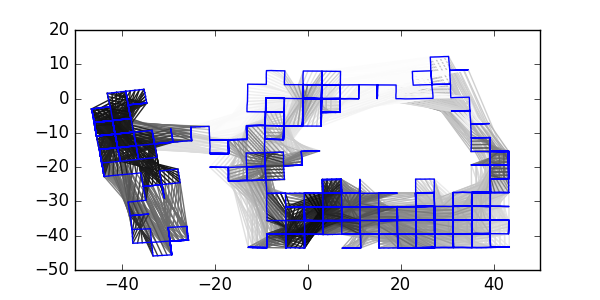
\includegraphics[width=0.33\textwidth,trim={1cm 0 1cm 0},clip]{figures/pose_pair_corr_y_100.png}
    }
    \subfloat[位姿对的相关性 - 航向(Heading)\label{fig:t_corr_100}]{%
       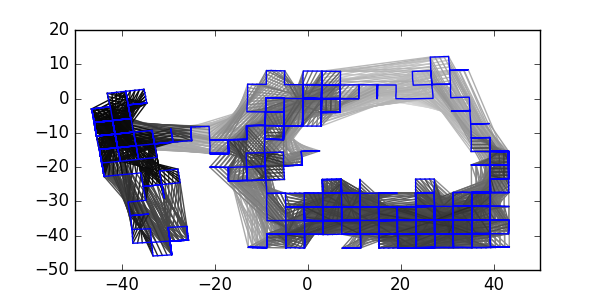
\includegraphics[width=0.33\textwidth,trim={1cm 0 1cm 0},clip]{figures/pose_pair_corr_t_100.png}
    }
    \hfill
    \subfloat[所提议的李代数相对位姿协方差误差\label{fig:joint_error_100}]{%
       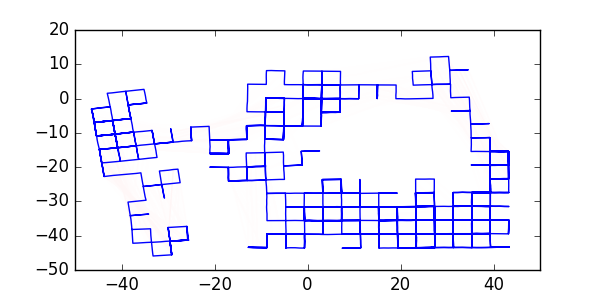
\includegraphics[width=0.39\textwidth,trim={1cm 0 1cm 0},clip]{figures/joint_relative_pose_cov_error_100.png}
    }
    \subfloat[所提议的李代数相对位姿协方差误差(忽略相关性)\label{fig:indep_error_100}]{%
       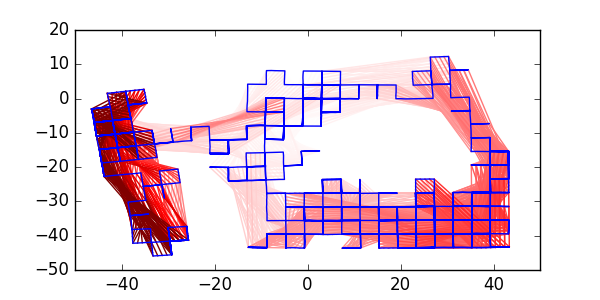
\includegraphics[width=0.39\textwidth,trim={1cm 0 1cm 0},clip]{figures/indep_relative_pose_cov_error_100.png}
    }\hfill
        \subfloat[所提议的李代数相对位姿归一化协方差误差\label{fig:norm_joint_error_100}]{%
       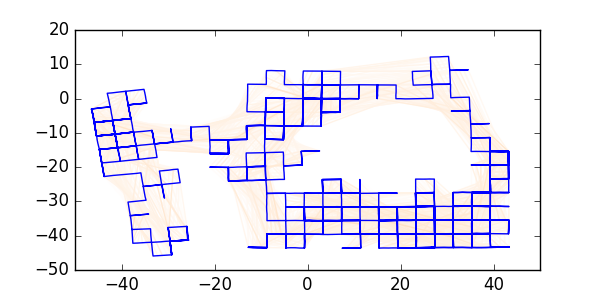
\includegraphics[width=0.39\textwidth,trim={1cm 0 1cm 0},clip]{figures/norm_joint_relative_pose_cov_error_100.png}
    }
    \subfloat[SSC 相对位姿归一化协方差误差\label{fig:norm_ssc_error_100}]{%
       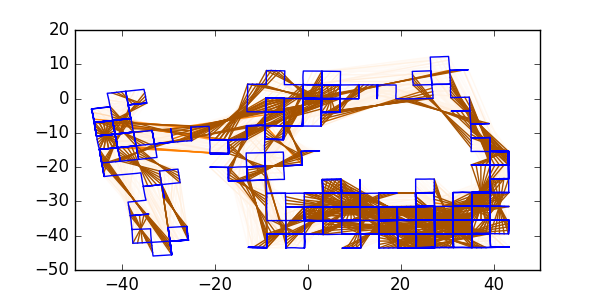
\includegraphics[width=0.39\textwidth,trim={1cm 0 1cm 0},clip]{figures/norm_ssc_relative_pose_cov_error_100.png}
    }\hfill
  \caption{从 Manhattan3500 数据集合 \cite{olson2006fast} 的解中提取的偏移量为100个节点的3400个位姿对的相关性和协方差误差的可视化图。配色方案与 \figref{fig:slam_rp_error_50} 的配色方案相匹配。}
  \label{fig:slam_rp_error_100}
\end{figure*}

\begin{figure*}[!t]%
    \centering%
    \subfloat[位姿对的相关性 - X\label{fig:x_corr_200}]{%
       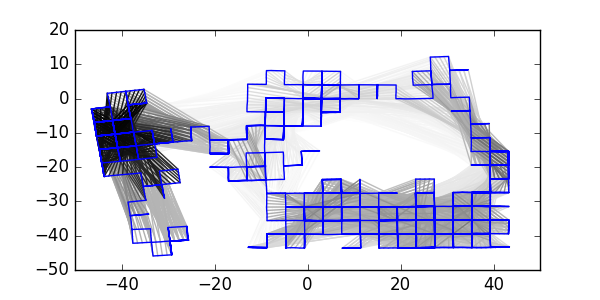
\includegraphics[width=0.33\textwidth,trim={1cm 0 1cm 0},clip]{figures/pose_pair_corr_x_200.png}
    }
    \subfloat[位姿对的相关性 - Y\label{fig:y_corr_200}]{%
       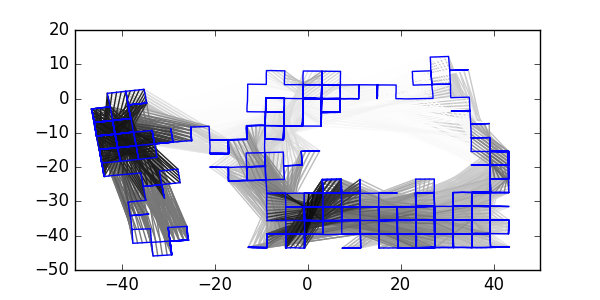
\includegraphics[width=0.33\textwidth,trim={1cm 0 1cm 0},clip]{figures/pose_pair_corr_y_200.png}
    }
    \subfloat[位姿对的相关性 - 航向(Heading)\label{fig:t_corr_200}]{%
       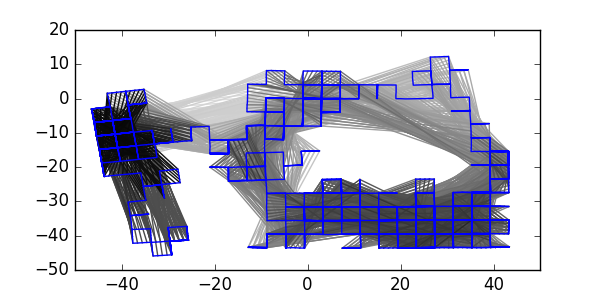
\includegraphics[width=0.33\textwidth,trim={1cm 0 1cm 0},clip]{figures/pose_pair_corr_t_200.png}
    }
    \hfill
    \subfloat[所提议的李代数相对位姿协方差误差\label{fig:joint_error_200}]{%
       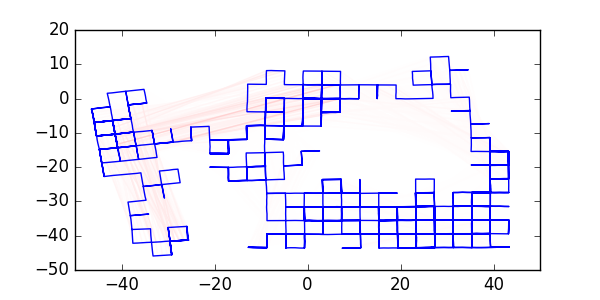
\includegraphics[width=0.39\textwidth,trim={1cm 0 1cm 0},clip]{figures/joint_relative_pose_cov_error_200.png}
    }
    \subfloat[所提议的李代数相对位姿协方差误差(忽略相关性)\label{fig:indep_error_200}]{%
       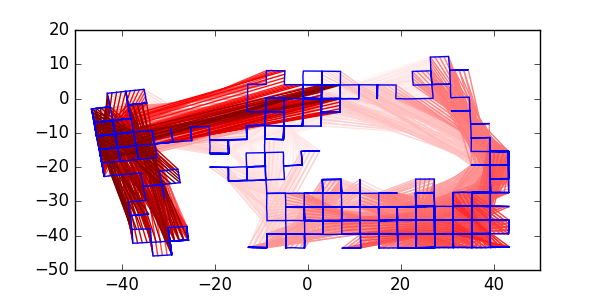
\includegraphics[width=0.39\textwidth,trim={1cm 0 1cm 0},clip]{figures/indep_relative_pose_cov_error_200.png}
    }\hfill
        \subfloat[所提议的李代数相对位姿归一化协方差误差\label{fig:norm_joint_error_200}]{%
       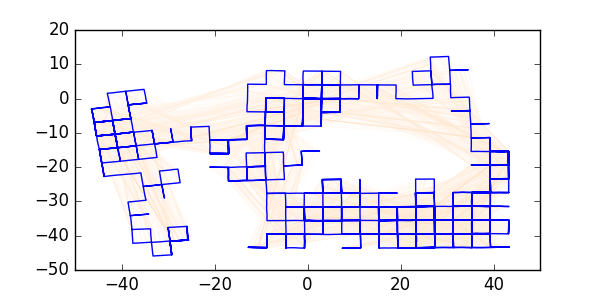
\includegraphics[width=0.39\textwidth,trim={1cm 0 1cm 0},clip]{figures/norm_joint_relative_pose_cov_error_200.png}
    }
    \subfloat[SSC 相对位姿归一化协方差误差\label{fig:norm_ssc_error_200}]{%
       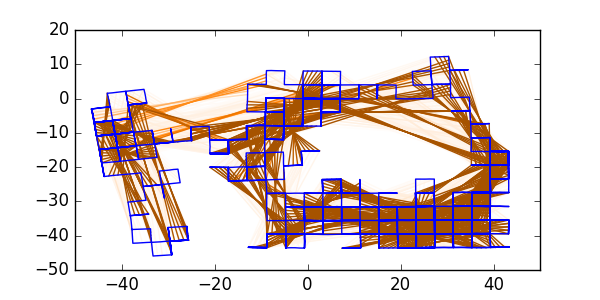
\includegraphics[width=0.39\textwidth,trim={1cm 0 1cm 0},clip]{figures/norm_ssc_relative_pose_cov_error_200.png}
    }\hfill
  \caption{从 Manhattan3500 数据集合 \cite{olson2006fast} 的解中提取的偏移量为200个节点的3300个位姿对的相关性和协方差误差的可视化图。配色方案与 \figref{fig:slam_rp_error_50} 的配色方案相匹配。}
  \label{fig:slam_rp_error_200}
\end{figure*}

\begin{figure*}[!t]%
    \centering%
    \subfloat[位姿对的相关性 - X\label{fig:x_corr_500}]{%
       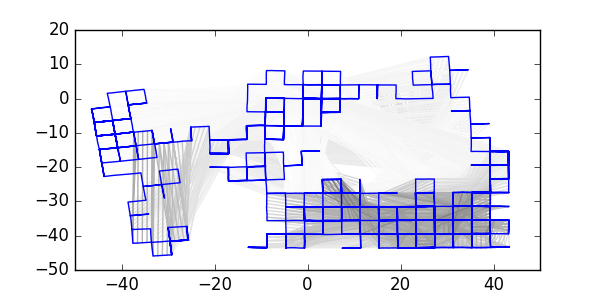
\includegraphics[width=0.33\textwidth,trim={1cm 0 1cm 0},clip]{figures/pose_pair_corr_x_500.png}
    }
    \subfloat[位姿对的相关性 - Y\label{fig:y_corr_500}]{%
       \includegraphics[width=0.33\textwidth,trim={1cm 0 1cm 0},clip]{figures/pose_pair_corr_y_500.png}
    }
    \subfloat[位姿对的相关性 - 航向(Heading)\label{fig:t_corr_500}]{%
       \includegraphics[width=0.33\textwidth,trim={1cm 0 1cm 0},clip]{figures/pose_pair_corr_t_500.png}
    }
    \hfill
    \subfloat[所提议的李代数相对位姿协方差误差\label{fig:joint_error_500}]{%
       \includegraphics[width=0.39\textwidth,trim={1cm 0 1cm 0},clip]{figures/joint_relative_pose_cov_error_500.png}
    }
    \subfloat[所提议的李代数相对位姿协方差误差(忽略相关性)\label{fig:indep_error_500}]{%
       \includegraphics[width=0.39\textwidth,trim={1cm 0 1cm 0},clip]{figures/indep_relative_pose_cov_error_500.png}
    }\hfill
        \subfloat[所提议的李代数相对位姿归一化协方差误差\label{fig:norm_joint_error_500}]{%
       \includegraphics[width=0.39\textwidth,trim={1cm 0 1cm 0},clip]{figures/norm_joint_relative_pose_cov_error_500.png}
    }
    \subfloat[SSC 相对位姿归一化协方差误差\label{fig:norm_ssc_error_500}]{%
       \includegraphics[width=0.39\textwidth,trim={1cm 0 1cm 0},clip]{figures/norm_ssc_relative_pose_cov_error_500.png}
    }\hfill
  \caption{从 Manhattan3500 数据集合 \cite{olson2006fast} 的解中提取的偏移量为500个节点的3000个位姿对的相关性和协方差误差的可视化图。配色方案与 \figref{fig:slam_rp_error_50} 的配色方案相匹配。}
  \label{fig:slam_rp_error_500}
\end{figure*}

%\begin{figure*}[!t]%
%    \centering%
%    \subfloat[Pose Pair Correlation - X\label{fig:x_corr_500}]{%
%       \includegraphics[width=0.33\textwidth,trim={1cm 0 1cm 0},clip]{figures/pose_pair_corr_x_500.png}
%    }
%    \subfloat[Pose Pair Correlation - Y\label{fig:y_corr_500}]{%
%       \includegraphics[width=0.33\textwidth,trim={1cm 0 1cm 0},clip]{figures/pose_pair_corr_y_500.png}
%    }
%    \subfloat[Pose Pair Correlation - Heading\label{fig:t_corr_500}]{%
%       \includegraphics[width=0.33\textwidth,trim={1cm 0 1cm 0},clip]{figures/pose_pair_corr_t_500.png}
%    }
%    \hfill
%    \subfloat[Joint Relative Pose Cov. Error\label{fig:joint_error_500}]{%
%       \includegraphics[width=0.45\textwidth,trim={1cm 0 1cm 0},clip]{figures/joint_relative_pose_cov_error_500.png}
%    }
%    \subfloat[Indep. Relative Pose Cov. Error\label{fig:indep_error_500}]{%
%       \includegraphics[width=0.45\textwidth,trim={1cm 0 1cm 0},clip]{figures/indep_relative_pose_cov_error_500.png}
%    }\hfill
%  \caption{A visualization of the correlation and covariance error for 3000 pose pairs with an offset of 500 nodes extracted from a solution of the Manhattan3500 dataset \cite{olson2006fast}. The color schemes match those of \figref{fig:slam_rp_error_50}}.
%  \label{fig:slam_rp_error_500}
%\end{figure*}

为了评估相对位姿的提取,我们使用 iSAM \cite{kaess2008isam} 来寻找 Manhattan3500 数据集合 \cite{olson2006fast} 的解。然后,我们按照在第 \secref{sec:convert:cov_extraction} 节中的描述,提取了偏移量从5到50,增量为5,以及偏移量为100、200和500的节点。所提取的位姿对和它们之间的相关性的可视化,在偏移量为50的情况下,显示在 \figref{fig:slam_rp_error_50} (a-c) 中。对于偏移量为10、100、200和500的情况,相同的可视化显示在 \figref{fig:slam_rp_error_10}、\figref{fig:slam_rp_error_100}、\figref{fig:slam_rp_error_200} 和 \figref{fig:slam_rp_error_500} 中。 

为了研究在估计相对位姿时考虑相关性的重要性,我们进行了蒙特卡洛模拟,以估计真实的相对位姿协方差,如在方程 \eqref{eq:sample_mc_cov} - \eqref{eq:sample_mc_xi} 中所描述的,其中 $\boldsymbol{\xi}_{g1}^{m}$ 和 $\boldsymbol{\xi}_{g2}^{m}$ 是从所提取的联合协方差中采样的扰动变量,并且 $\bar{\mathbf{T}}_{g1}$ 和 $\bar{\mathbf{T}}_{g2}$ 是从 iSAM 的解中提取的均值。然后,我们使用在方程 \eqref{eq:cov_error} 中定义的度量来评估在方程 \eqref{eq:relative_pose_cov} 中我们所提议的方法,在考虑相关性(使用方程 \eqref{eq:relative_pose_cov} 中的所有四项)或忽略相关性(仅使用方程 \eqref{eq:relative_pose_cov} 中的前两项)时的协方差误差。摘要统计信息如表 \ref{table:cov_error} 中所示,并且偏移量为50、10、100、200和500时的误差可视化显示在 \figref{fig:slam_rp_error_50},\figref{fig:slam_rp_error_10},\figref{fig:slam_rp_error_100},\figref{fig:slam_rp_error_200},和 \figref{fig:slam_rp_error_500} 的 (d-e) 子图中。 

表 \ref{table:cov_error} 中的结果表明,忽略相关性会导致协方差误差比考虑相关性时高出$3$个数量级以上。 

为了将我们所提议的方法与 SSC \cite{smith1990a} 进行比较,我们进行了一个类似的实验,不同的是,SSC的的蒙特卡洛的“真实数据”协方差是通过从先前的实验中获取样本相对位姿,并将其转换为方程 \eqref{eq:SSC_rep} 中描述的参数向量格式,并获取样本协方差而得到的。为了公平地比较我们所提议的方法与 SSC,在评估在方程 \eqref{eq:cov_error} 中定义的协方差误差之前,用蒙特卡洛协方差矩阵的Frobenious范数对协方差矩阵进行归一化。实验总结统计显示在表 \ref{table:norm_cov_error} 中,并且偏移量为50、10、100、200和500时的误差可视化显示在 \figref{fig:slam_rp_error_50},\figref{fig:slam_rp_error_10},\figref{fig:slam_rp_error_100},\figref{fig:slam_rp_error_200},和 \figref{fig:slam_rp_error_500} 的 (f-g) 的子图中。 

应该注意的是,这不是一个完美的比较,因为与SSC比较的蒙特卡洛协方差是一个多元高斯拟合的参数向量集合,不能精确地建模为高斯分布。然而,结果确实表明,即使以SSC表示法所假设的格式对真实误差进行建模,我们所提议的基于李代数的方法所产生的协方差误差也比SSC低一个数量级(参见表 \ref{table:norm_cov_error})。 

\section{代码库的实现}
\label{sec:library}

我们已经发布了一个实现我们的方法的开源C++库。它可以从这里下载:https://bitbucket.org/jmangelson/lie。我们试图把它设计成简单、直观、易于扩展的。 

\subsection{创建已知和不确定的 $\mathrm{SE}(3)$ 对象}

创建已知和不确定的 $\mathrm{SE}(3)$ 对象在语法上很容易。 
导入库之后,可以使用各种构造函数来创建已知的 $\mathrm{SE}(3)$ 的变换: 
\begin{verbatim}
#include <lie/se3.hpp>

// Via rotation and translation 
Eigen::MatrixXd R(3,3); // 3x3 matrix 
Eigen::VectorXd t(3); // 3x1 vector
Lie::SE3 T_12(R, t);    
    
// Via translation and Euler angle params
Lie::SE3 T_23(x, y, z, theta, phi, psi);
\end{verbatim}

通过传入均值或均值元组以及协方差矩阵,还可以创建未知位姿的独立且联合分布的集合。 
\begin{verbatim}
Lie::SE3 T_ab_mu(R_ab, t_ab);  
Eigen::MatrixXd Sigma_ab(6,6);
auto T_ab_uncertain = 
  Lie::make_uncertain_state(
    T_ab_mu, Sigma_ab);
   
Lie::SE3 T_ac_mu(R_ac, t_ac);  
Eigen::MatrixXd Sigma_Joint(12,12);
auto refs = 
  Lie::make_uncertain_state(
    std::make_tuple(T_ab_mu, T_ac_mu), 
    Sigma_Joint);
auto T_ab_uncertain = std::get<0>(refs);
auto T_ac_uncertain = std::get<1>(refs);
\end{verbatim}

这个 \texttt{Lie::make\_uncertain\_state} 函数返回单个 $\mathrm{SE}(3)$ 引用对象或这样的对象的元组,这些对象可以用来执行操作。

\subsection{执行操作}

位姿组合、求逆和相对位姿操作可以无条件地可互换地应用,而不管已知或不确定的 $\mathrm{SE}(3)$ 对象是否分别通过 \texttt{Lie::compose}、\texttt{inverse} 和 \texttt{Lie::between} 函数获取。 
编译器自动确定单个对象是已知/未知还是独立/联合分布,并应用适当的公式。 

\begin{verbatim}
// Composing known poses
auto T_13 = Lie::compose(T_12, T_23);
  
// Invert both known and uncertain poses
auto T_21 = T_12.inverse();
auto T_ba_uncertain = 
  T_ab_uncertain.inverse();
  
// Calculating relative pose
auto T_bc_uncertain = Lie::between(
  T_ab_uncertain, T_ac_uncertain);
auto T_bc_uncertain2 = Lie::between(
  T_ab_known, T_ac_uncertain);
\end{verbatim}

每个函数返回一个新的(从那时起假定是独立的) $\mathrm{SE}(3)$ 引用对象,可以根据需要用于其它操作。 

\subsection{其它李群类}

另外,由于本文提出的不确定性传播方法简单地利用了李群的性质,因此可以很容易地应用于其它类型的李群。 
我们还为 $\mathrm{SO}(3)$、$\mathrm{SE}(2)$ 和 $\mathrm{SO}(2)$ 的李群实现了 \texttt{Lie::SO3}、\texttt{Lie::SE2} 和 \texttt{Lie::SE2} 这些类,并计划根据需要将其扩展到其它李群类型。 

%
\section{\normalfont\bfseries 结果 \label{sec:Results}}

为了评估对偶四元数牛顿-欧拉形式(dual quaternion Newton-Euler, dqNE)和使用对偶四元数高斯最小约束原理(dual quaternion Gauss's Principle, dqGP)得到的欧拉-拉格朗日模型,我们使用三个不同的机器人进行了仿真;即一个固定基座 $50$ 自由度串联机械手、一个 $9$ 自由度完整移动机械臂和一个 $8$ 自由度非完整移动机械臂。

我们在机器人模拟器 ${\text{V-REP PRO EDU V3.6.2}}$ 上\footnote{可在以下网址获得: https://www.coppeliarobotics.com/}进行了模拟,其使用 Matlab 2020a 接口和对偶四元数代数计算库DQ Robotics \cite{AdornoDQRobotics2020},运行在Ubuntu 18.04 LTS 64 位(配备Intel Core i7 6500U和8GB RAM)的计算机上。 

此外,我们给出了所提议方法的计算成本,并将其与各自的经典方法进行了比较。

\subsection{\normalfont\bfseries 模拟设置}

考虑到波形之间的多重相关系数(coefficient of multiple correlation, CMC) \cite{Ferrari2010},通过我们提出的模型获得的广义加速度与来自V-REP的值之间进行了比较。CMC提供介于0和1之间的系数,指示两个给定波形的相似程度。相同波形的CMC等于1,而完全不同的波形的CMC等于0。

模拟器不允许直接读取加速度。因此,为了获得位形加速度向量 $\ddot{\myvec q}$,我们首先读取速度向量 $\dot{\myvec q}\in\mathbb{R}^{n_{\ell}+3}$,然后使用离散低通Butterworth滤波器过滤所有元素 $\dot{q}_{1},\ldots,\dot{q}_{n_{\ell}+3}$,并使用这些值通过数值微分方法以获得加速度,该方法基于一个第二次正向有限差分近似的算法。然后,我们计算了广义加速度波形的每个元素 $\ddot{q}_{i}$,其中$i\in\{1,\ldots,n_{\ell}+3\}$,并计算与V-REP的对应元素之间的CMC。之后,我们使用这些CMC获得模型的平均值、最小值和最大值以及它们的标准偏差。

此外,对于固定基座 $50$ 自由度串联机械臂的模拟,我们还使用了Robotics Toolbox \cite{Corke2017} 以实现的经典的递归牛顿-欧拉算法(recursive Newton-Euler, rtNE),并计算了它产生的关节加速度波形与V-REP产生的关节加速度波形之间的CMC。\footnote{在本例中,我们使用 Vortex Studio 引擎 (www.cm-labs.com),因为它为 $50$ 自由度机械臂提供了更好的数值稳定性。}机器人工具箱是一个广泛使用的软件库,其准确性多年来一直得到验证。因此,它是评估通过使用我们的模型获得的CMC的适当基准。

\subsection{\normalfont\bfseries 结果}

表~\ref{tab:cmc} 显示了通过不同动力学模型策略 (dqNE, dqGP, and rtNE) 获得的广义加速度波形与从V-REP获得的值之间的 CMC。

所提议的对偶四元数牛顿-欧拉形式不允许在模型中包含等式约束;因此,它不适用于非完整移动机械臂的动力学建模。同样,当前版本的Robotics Toolbox仅支持固定基座机器人的动力学建模,仅适用于 $50$ 自由度串联机械臂。使用所列策略无法获得模型的情况如表~\ref{tab:cmc} 所示,用 N/A 表示,(即,不可用)即不可用。对于所有其他情况,所有模型的平均值 ($\mathrm{mean}$) 和最小值 ($\mathrm{min}$) 的CMC接近1,具有小的标准偏差 ($\mathrm{std}$) 和高的最大值 $\left(\mathrm{max}\right)$ 的 CMC;由此表明,由它们得到的广义加速度波形与来自V-REP的值具有高度的相似性。

\begin{table*}[t]
\caption{通过不同动力学模型策略获得的关节加速度波形与通过V-REP获得的值之间的CMC。越接近1,波形越相似。\label{tab:cmc}}

\centering{}{\small{}}%
\begin{tabular}{cc|cccc|cccc|cccc}
\hline 
 & \multicolumn{1}{c}{} & \multicolumn{4}{c}{{\small{}\hspace{1mm}$50$自由度串联机械臂}} & \multicolumn{4}{c}{{\small{}$9$自由度完整移动机械臂}} & \multicolumn{4}{c}{{\small{}~~$8$自由度非完整移动机械臂~~}}\tabularnewline
\hline 
{\small{}~~~~~Method~~~~~} &  & {\small{}\hspace{4mm}min\hspace{4mm}} & {\small{}\hspace{4mm}mean\hspace{4mm}} & {\small{}\hspace{4mm}std\hspace{4mm}} & {\small{}\hspace{4mm}max\hspace{4mm}} & {\small{}\hspace{4mm}min\hspace{4mm}} & {\small{}\hspace{4mm}mean\hspace{4mm}} & {\small{}\hspace{4mm}std\hspace{4mm}} & {\small{}\hspace{4mm}max\hspace{4mm}} & {\small{}\hspace{4mm}min\hspace{4mm}} & {\small{}\hspace{4mm}mean\hspace{4mm}} & {\small{}\hspace{4mm}std\hspace{4mm}} & {\small{}\hspace{4mm}max~~~~~}\tabularnewline
\hline 
\multicolumn{2}{c|}{{\small{}dqGP~~~}} & {\small{}$0.9044$} & {\small{}$0.9893$} & {\small{}$0.0182$} & {\small{}$0.9993$} & {\small{}$0.9934$} & {\small{}$0.9973$} & {\small{}$0.0026$} & {\small{}$0.9999$} & {\small{}$0.8860$} & {\small{}$0.9839$} & {\small{}$0.0368$} & {\small{}$0.9999$}\tabularnewline
\multicolumn{2}{c|}{{\small{}dqNE~~~}} & {\small{}$0.9044$} & {\small{}$0.9893$} & {\small{}$0.0182$} & {\small{}$0.9993$} & {\small{}$0.9938$} & {\small{}$0.9977$} & {\small{}$0.0022$} & {\small{}$0.9999$} & {\small{}N/A} & {\small{}N/A} & {\small{}N/A} & {\small{}N/A}\tabularnewline
\multicolumn{2}{c|}{{\small{}rtNE~~}} & {\small{}$0.9044$} & {\small{}$0.9893$} & {\small{}$0.0182$} & {\small{}$0.9993$} & {\small{}N/A} & {\small{}N/A} & {\small{}N/A} & {\small{}N/A} & {\small{}N/A} & {\small{}N/A} & {\small{}N/A} & {\small{}N/A}\tabularnewline
\hline 
\end{tabular}{\small\par}
\end{table*}

对于 $50$自由度串联机械臂,dqNE和dqGP均等效于rtNE,这证明了与经典的牛顿-欧拉方法相比,我们所提议的策略的准确性。

对于定性分析,图~\ref{fig:joint_acc_nonholonomic_jaco} 显示了在模拟过程中发现的最小、最大和中间的CMC时,使用dqGP获得的广义加速度,以及V-REP的值。即使对于CMC的最小值(即0.8860),使用我们的公式获得的加速度也与V-REP的值非常匹配。小的差异产生于两个原因,一是离散化效应,二是因为V-REP中的加速度从有噪声的速度值估计。

\begin{figure}[t]
\begin{centering}
{\Huge{}\resizebox{0.93\columnwidth}{!}{\input{Images/results_accel/joint_acc_nonholonomic_jaco.pdf_tex}}}{\Huge\par}
\par\end{centering}
\caption{$8$自由度非完整移动机械臂产生的广义加速度波形。实线曲线对应于V-REP值,而点划线曲线对应于使用dqGP分别获得的第一个 ($\text{CMC}=0.8860$)、第九个 ($\text{CMC}=0.9999$)和第五个 ($\text{CMC}=0.9922$) 关节的广义加速度波形值。\label{fig:joint_acc_nonholonomic_jaco}}
\end{figure}


\subsection{\normalfont\bfseries 计算成本}

在这里,我们将所提议的方法与经典方法在每种技术中涉及的乘法和加法的数量方面进行比较。其结果,考虑了 \emph{n} 自由度的串行机器人,汇总在表~\ref{tab:summary_cost_table-1} 中。对于经典的牛顿-欧拉算法,我们考虑 Luh 等人 \cite{Luh1980} 提出的基于三维向量的版本,其数学成本由 Balafoutis \cite{Balafoutis1994} 计算,并且据我们所知,这是文献中最有效的实现之一。此外,对于经典的欧拉-拉格朗日算法,我们考虑的是由 Hollerbach \cite{Hollerbach1980} 所提出的版本。

\begin{table*}[t]
\noindent \centering{}\caption{对于 \emph{n} 自由度串联机器人,对于所获得的动力学模型,所提议的方法与经典方法的成本比较。
\label{tab:summary_cost_table-1}}
{\small{}}%
\begin{tabular*}{1\textwidth}{@{\extracolsep{\fill}}lcc}
\hline 
{\small{}方法} & {\small{}乘法数量} & {\small{}加法数量}\tabularnewline
\hline 
{\small{}\makecell[l]{对偶四元数牛顿-欧拉算法 \\(对于任意关节的成本)}} & {\small{}$882n-48$} & {\small{}$724n-40$}\tabularnewline
{\small{}经典牛顿-欧拉算法 \cite{Balafoutis1994}} & {\small{}$150n-48$} & {\small{}$131n-48$}\tabularnewline
{\small{}\makecell[l]{对偶四元数欧拉-拉格朗日算法 \\使用高斯最小约束原理}} & \multirow{1}{*}{{\small{}$4n^{3}+386n^{2}+401n$}} & \multirow{1}{*}{{\small{}$\frac{16}{3}n^{3}+326n^{2}+\frac{908}{3}n$}}\tabularnewline
{\small{}经典欧拉-拉格朗日算法 \cite{Hollerbach1980}} & \multirow{1}{*}{{\small{}$412n-277$}} & \multirow{1}{*}{{\small{}$320n-201$}}\tabularnewline
\hline 
\end{tabular*}
\end{table*}

Luh等人 \cite{Luh1980} 提出的算法比我们的对偶四元数牛顿-欧拉算法成本更低。然而,我们提出的方法的成本是相当保守的,并且是作为一个上限给出的。例如,我们的计算可以通过探索一些事实来进一步优化,其中有几个运算涉及纯对偶四元数,可由八个元素改为六个元素。此外,Balafoutis \cite{Balafoutis1994} 提出的成本不包括获取机器人运动学模型的成本。另外,我们的方法适用于\textbf{任意}类型的关节,并且我们没有优化任意特定类型关节的计算,这与Luh等人 \cite{Luh1980} 不同,他们只考虑了棱柱关节和旋转关节,这被利用以优化计算成本。尽管如此,我们的算法和Luh等人的算法都在自由度数量上具有线性成本,其系数的数量级都相同。

基于高斯最小约束原则的欧拉-拉格朗日方法,与基于基于牛顿-欧拉和经典欧拉-拉格朗日的方法相比,成本更高,正如预期的那样,因为它不是基于递归策略的。然而,这种策略允许考虑加速度中的附加约束,例如,在非完整机器人系统中可以利用。对于这些情况,欧拉-拉格朗日动力学方程由方程  \eqref{eq:FinalGaussUK} 给出。


\section{\normalfont\bfseries 结论\label{sec:Conclusions}}

本项工作对于基于对偶四元数代数的移动机械臂动力学模型的表示方法,提出了两种策略。第一种是基于递归牛顿-欧拉公式,并使用运动旋量和动力旋量代替自由向量。这种表示方法消除了对运动链进行详尽几何分析的必要性,因为动力旋量和运动旋量是通过高级代数运算传播的。此外,我们的公式适用于任意类型的关节,因为它考虑了任意运动旋量。因此,我们的策略比Miranda等人\cite{MirandadeFarias2019Journal}的工作更一般,他们只考虑具有旋转关节的机械臂。

第二种方法基于高斯最小约束原理,并且它也被制定基于对偶四元数代数所表示的运动旋量和动力旋量的矩阵形式,该策略允许在优化公式中直接加入等式约束。

所提议方法与经典方法的成本比较表明,在乘法和加法次数方面,对偶四元数的使用不会显著增加牛顿-欧拉形式的成本,因为该算法对运动链中的刚体数量具有线性复杂度。然而,使用高斯最小约束原理和对偶四元数代数得到欧拉-拉格朗日模型的成本高于在文献中发现的最佳经典欧拉-拉格朗日递推解。尽管如此,我们的方法远比这些经典的方法更通用。另外,我们没有做出任何努力来优化我们的实现(如果有的话),因为我们目前更感兴趣的是使用对偶四元数代数进行动态建模的理论方面,而不是确保计算效率。在我们目前的MATLAB实现中,dqNE和dqGP平均分别需要 23.17s 和 8.73s 以产生$50$自由度机械臂机器人的关节加速度。在C++实现中,这些值预计将分别减少到 99 ms 和 37 ms 左右 \cite{AdornoDQRobotics2020}。

通过牛顿-欧拉形式获得欧拉-拉格朗日模型需要多次执行该算法。一次执行以获得重力向量,一次执行以获得科里奥利项和离心项的向量,并且对于惯量矩阵 $\mymatrix M$ 的每一行都执行一次。对于一个$50$自由度机械臂的机器人,每个模拟步骤执行 $52$ 次dqNE。然而,对于控制应用,我们通常是对寻找关节扭矩感兴趣,它只需要执行一次dqNE以产生每个控制输入。因此,使用dqNE计算$50$自由度机械臂机器人的关节扭矩,在C++实现中,执行时间预计将减少 $52$ 倍,从大约 99~ms 减少到 1.9~ms。

最后,对于三种不同机器人,我们通过提议的策略获取的关节加速度,与从 ${\text{V-REP PRO EDU V3.6.2}}$ (一个真实的模拟器)中获取的值进行了比较。结果表明,我们所有的方法对于固定基座串联机械臂和移动机械臂都是精确的。

未来的工作重点是将对偶四元数牛顿-欧拉算法推广到非串联多体系统(如仿人系统),以及动力旋量控制策略中。对于使用高斯最小约束原理和对偶四元数代数获得的欧拉-拉格朗日模型,未来的工作将集中于在优化表示方法中运用不等式约束。



%\footnotesize
\balance
\bibliographystyle{style/IEEEtranN}
{\footnotesize
\bibliography{references/IEEEabrv,references/strings-short,%
    references/library}}


%\FloatBarrier
\begin{IEEEbiography}[{\includegraphics[width=1in,height=1.25in,clip,keepaspectratio]{figures/jman_small.jpg}}]{Joshua Mangelson}

%(S'13) 
received the B.S. degree in electrical engineering from Brigham Young University, Provo, UT, USA in 2014 and the M.S. degree in robotics from the University of Michigan, Ann Arbor, MI, USA in 2016. He is currently a Ph.D. candidate in robotics at the University of Michigan with expected completion in April 2019. His research interests lie in the development of navigation, mapping, perception, and planning algorithms with mathematical and performance guarantees that enable the design of reliable field robotic systems for operation in unstructured environments. He is especially interested in the development of large-scale multi-agent teams for autonomous inspection of underwater structures. He is the recipient of the IEEE ICRA Best Multi-Robot Paper Award and the IEEE OCEANS Best Poster Award both in 2018. 
\end{IEEEbiography}

\vspace{-2 cm}

\begin{IEEEbiography}[{\includegraphics[width=1in,height=1.25in,clip,trim={4.7cm 0 5.7cm 0},keepaspectratio]{figures/mgj.jpg}}]{Maani Ghaffari}

%() 
received the Ph.D. degree from the Centre for Autonomous Systems (CAS), University of Technology Sydney, NSW, Australia, in 2017. He is currently an Assistant Research Scientist at the Robotics Institute and Department of Naval Architecture and Marine Engineering, University of Michigan, Ann Arbor, MI, USA. His research interests include applied mathematics, robotic perception, machine learning, and planning under uncertainty with applications in robotics and autonomous systems.
\end{IEEEbiography}

\begin{IEEEbiography}[{\includegraphics[width=1in,height=1.25in,clip,trim={0 0.03cm 0 0},keepaspectratio]{figures/RamVasudevan.JPG}}]{Ram Vasudevan}

%() 
received the B.S. degree in electrical engineering and computer sciences, the M.S. degree in electrical engineering, and the Ph.D. degree in electrical engineering from the University of California at Berkeley in 2006, 2009, and 2012, respectively.
He is currently an Assistant Professor in mechanical engineering with the University of Michigan, Ann Arbor, with an appointment in the University of Michigan’s Robotics Program. His research interests include the development and application of optimization and systems theory to quantify and improve human and robot interaction.
\end{IEEEbiography}

\vspace{-1 cm}

\begin{IEEEbiography}[{\includegraphics[width=1in,height=1.25in,clip,trim={1.1cm 0 0.1cm 0},keepaspectratio]{figures/RME.jpg}}]{Ryan M. Eustice}

%(S'00-M'05-SM'10) 
received the B.S. degree in mechanical engineering from Michigan State University, East Lansing, MI, USA, in 1998 and the Ph.D. degree in ocean engineering from the Joint Program between the Massachusetts Institute of Technology (MIT), Cambridge, MA, USA and the Woods Hole Oceanographic Institution (WHOI), Woods Hole, MA, USA, in 2005. Currently, he is the Senior Vice President of Automated Driving at the Toyota Research Institute and a Professor with the Department of Naval Architecture and Marine Engineering, University of Michigan, Ann Arbor, MI, USA, with joint appointments in the Department of Electrical Engineering and Computer Science and in the Department of Mechanical Engineering. His research interests include autonomous navigation and mapping, automated driving, mobile robotics, and autonomous underwater vehicles.

\end{IEEEbiography}

% that's all folks
\end{document}

 
